%%%%%%%%%%%%%%%%%%%%%%%%%%%%%%%%%%%%%%%%%
% The Legrand Orange Book
% LaTeX Template
% Version 2.4 (26/09/2018)
%
% This template was downloaded from:
% http://www.LaTeXTemplates.com
%
% Original author:
% Mathias Legrand (legrand.mathias@gmail.com) with modifications by:
% Vel (vel@latextemplates.com)
%
% License:
% CC BY-NC-SA 3.0 (http://creativecommons.org/licenses/by-nc-sa/3.0/)
%
% Compiling this template:
% This template uses biber for its bibliography and makeindex for its index.
% When you first open the template, compile it from the command line with the 
% commands below to make sure your LaTeX distribution is configured correctly:
%
% 1) pdflatex main
% 2) makeindex main.idx -s StyleInd.ist
% 3) biber main
% 4) pdflatex main x 2
%
% After this, when you wish to update the bibliography/index use the appropriate
% command above and make sure to compile with pdflatex several times 
% afterwards to propagate your changes to the document.
%
% This template also uses a number of packages which may need to be
% updated to the newest versions for the template to compile. It is strongly
% recommended you update your LaTeX distribution if you have any
% compilation errors.
%
% Important note:
% Chapter heading images should have a 2:1 width:height ratio,
% e.g. 920px width and 460px height.
%
%%%%%%%%%%%%%%%%%%%%%%%%%%%%%%%%%%%%%%%%%

%----------------------------------------------------------------------------------------
%	PACKAGES AND OTHER DOCUMENT CONFIGURATIONS
%----------------------------------------------------------------------------------------

\documentclass[11pt,fleqn,twoside]{book} % Default font size and left-justified equations

%%%%%%%%%%%%%%%%%%%%%%%%%%%%%%%%%%%%%%%%%
% The Legrand Orange Book
% Structural Definitions File
% Version 2.1 (26/09/2018)
%
% Original author:
% Mathias Legrand (legrand.mathias@gmail.com) with modifications by:
% Vel (vel@latextemplates.com)
% 
% This file was downloaded from:
% http://www.LaTeXTemplates.com
%
% License:
% CC BY-NC-SA 3.0 (http://creativecommons.org/licenses/by-nc-sa/3.0/)
%
%%%%%%%%%%%%%%%%%%%%%%%%%%%%%%%%%%%%%%%%%

%----------------------------------------------------------------------------------------
%	VARIOUS REQUIRED PACKAGES AND CONFIGURATIONS
%----------------------------------------------------------------------------------------

\usepackage{graphicx} % Required for including pictures
\graphicspath{{Pictures/}} % Specifies the directory where pictures are stored
\usepackage{subfig}
\usepackage{tikz} % Required for drawing custom shapes
\usepackage{PSTricks}
\usepackage[english]{babel} % English language/hyphenation

\usepackage{enumitem} % Customize lists
\setlist{nolistsep} % Reduce spacing between bullet points and numbered lists

\usepackage{booktabs} % Required for nicer horizontal rules in tables

\usepackage{xcolor} % Required for specifying colors by name
\definecolor{ocre}{RGB}{243,102,25} % Define the orange color used for highlighting throughout the book

%----------------------------------------------------------------------------------------
%	MARGINS
%----------------------------------------------------------------------------------------

\usepackage{geometry} % Required for adjusting page dimensions and margins
\geometry{
	paper=a4paper, % Paper size, change to letterpaper for US letter size
	top=3cm, % Top margin
	bottom=3cm, % Bottom margin
	inner=3cm, % Left margin
	outer=5cm, % Right margin
	headheight=14pt, % Header height
	footskip=1.4cm, % Space from the bottom margin to the baseline of the footer
	headsep=10pt, % Space from the top margin to the baseline of the header
	%showframe, % Uncomment to show how the type block is set on the page
}

%----------------------------------------------------------------------------------------
%	FONTS
%----------------------------------------------------------------------------------------
\usepackage[UTF8]{ctex}
\setCJKmainfont[Path=fonts/,BoldFont={SourceHanSerifCN-Bold.otf},ItalicFont={simkai.ttf}]{SourceHanSerifCN-Regular.otf}
\setCJKsansfont[Path=fonts/,BoldFont={SourceHanSansSC-Bold.otf}]{SourceHanSansSC-Regular.otf}
\usepackage{avant} % Use the Avantgarde font for headings
%\usepackage{times} % Use the Times font for headings
\usepackage{mathptmx} % Use the Adobe Times Roman as the default text font together with math symbols from the Sym­bol, Chancery and Com­puter Modern fonts

\usepackage{microtype} % Slightly tweak font spacing for aesthetics
\usepackage[utf8]{inputenc} % Required for including letters with accents
\usepackage[T1]{fontenc} % Use 8-bit encoding that has 256 glyphs

%---------------------------------------------------------------------------------------
% use sidenotes but fix its bug to change font size
% see: https://tex.stackexchange.com/questions/532245/how-to-modify-fonts-in-sidenotes
%---------------------------------------------------------------------------------------
\usepackage{sidenotes}
\usepackage{xparse}
\let\oldmarginpar\marginpar
\RenewDocumentCommand{\marginpar}{om}{%
	\IfNoValueTF{#1}
	{\oldmarginpar{\mymparsetup #2}}
	{\oldmarginpar[\mymparsetup #1]{\mymparsetup #2}}}
\newcommand{\mymparsetup}{\scriptsize\itshape}

%---------------------------------------------------------------------------------------
% use \eg ... see: https://stackoverflow.com/a/39363004/12128185
%---------------------------------------------------------------------------------------
\usepackage{xspace}
\makeatletter
\DeclareRobustCommand\onedot{\futurelet\@let@token\@onedot}
\def\@onedot{\ifx\@let@token.\else.\null\fi\xspace}
\def\eg{\emph{e.g}\onedot} \def\Eg{\emph{E.g}\onedot}
\def\ie{\emph{i.e}\onedot} \def\Ie{\emph{I.e}\onedot}
\def\cf{\emph{c.f}\onedot} \def\Cf{\emph{C.f}\onedot}
\def\etc{\emph{etc}\onedot} \def\vs{\emph{vs}\onedot}
\def\wrt{w.r.t\onedot} \def\dof{d.o.f\onedot}
\def\etal{\emph{et al}\onedot}
\makeatother

%----------------------------------------------------------------------------------------
%	BIBLIOGRAPHY AND INDEX
%----------------------------------------------------------------------------------------

\usepackage[style=authoryear,citestyle=authoryear,uniquename=init,sorting=nyt,sortcites=true,autopunct=true,babel=hyphen,hyperref=true,abbreviate=false,backref=true,backend=biber,natbib=true]{biblatex}
\addbibresource{bibliography.bib} % BibTeX bibliography file
\defbibheading{bibempty}{}

\usepackage{calc} % For simpler calculation - used for spacing the index letter headings correctly
\usepackage{makeidx} % Required to make an index
\makeindex % Tells LaTeX to create the files required for indexing
\usepackage{xifthen} % provides \isempty test
\newcommand\keyindex[3]{\ifthenelse{\isempty{#1}}{}{\ifthenelse{\isempty{#2}}{\ifthenelse{\isempty{#3}}{{\sffamily#1}}{{\sffamily#1}\index{#3!#1}}}{\ifthenelse{\isempty{#3}}{{\sffamily#1}(#2)\index{#2#1}}{{\sffamily#1}(#2)\index{#3!#2#1}}}}}

%----------------------------------------------------------------------------------------
%	MAIN TABLE OF CONTENTS
%----------------------------------------------------------------------------------------

\usepackage{titletoc} % Required for manipulating the table of contents

\contentsmargin{0cm} % Removes the default margin

% Part text styling (this is mostly taken care of in the PART HEADINGS section of this file)
\titlecontents{part}
[0cm] % Left indentation
{\addvspace{20pt}\bfseries} % Spacing and font options for parts
{}
{}
{}

% Chapter text styling
\titlecontents{chapter}
[1.25cm] % Left indentation
{\addvspace{12pt}\large\sffamily\bfseries} % Spacing and font options for chapters
{\color{ocre!60}\contentslabel[\Large\thecontentslabel]{1.25cm}\color{ocre}} % Formatting of numbered sections of this type
{\color{ocre}} % Formatting of numberless sections of this type
{\color{ocre!60}\normalsize\;\titlerule*[.5pc]{.}\;\thecontentspage} % Formatting of the filler to the right of the heading and the page number

% Section text styling
\titlecontents{section}
[1.25cm] % Left indentation
{\addvspace{3pt}\sffamily\bfseries} % Spacing and font options for sections
{\contentslabel[\thecontentslabel]{1.25cm}} % Formatting of numbered sections of this type
{} % Formatting of numberless sections of this type
{\hfill\color{black}\thecontentspage} % Formatting of the filler to the right of the heading and the page number

% Subsection text styling
\titlecontents{subsection}
[1.25cm] % Left indentation
{\addvspace{1pt}\sffamily\small} % Spacing and font options for subsections
{\contentslabel[\thecontentslabel]{1.25cm}} % Formatting of numbered sections of this type
{} % Formatting of numberless sections of this type
{\ \titlerule*[.5pc]{.}\;\thecontentspage} % Formatting of the filler to the right of the heading and the page number

% Figure text styling
\titlecontents{figure}
[1.25cm] % Left indentation
{\addvspace{1pt}\sffamily\small} % Spacing and font options for figures
{\thecontentslabel\hspace*{1em}} % Formatting of numbered sections of this type
{} % Formatting of numberless sections of this type
{\ \titlerule*[.5pc]{.}\;\thecontentspage} % Formatting of the filler to the right of the heading and the page number

% Table text styling
\titlecontents{table}
[1.25cm] % Left indentation
{\addvspace{1pt}\sffamily\small} % Spacing and font options for tables
{\thecontentslabel\hspace*{1em}} % Formatting of numbered sections of this type
{} % Formatting of numberless sections of this type
{\ \titlerule*[.5pc]{.}\;\thecontentspage} % Formatting of the filler to the right of the heading and the page number

%----------------------------------------------------------------------------------------
%	MINI TABLE OF CONTENTS IN PART HEADS
%----------------------------------------------------------------------------------------

% Chapter text styling
\titlecontents{lchapter}
[0em] % Left indentation
{\addvspace{15pt}\large\sffamily\bfseries} % Spacing and font options for chapters
{\color{ocre}\contentslabel[\Large\thecontentslabel]{1.25cm}\color{ocre}} % Chapter number
{}
{\color{ocre}\normalsize\sffamily\bfseries\;\titlerule*[.5pc]{.}\;\thecontentspage} % Page number

% Section text styling
\titlecontents{lsection}
[0em] % Left indentation
{\sffamily\small} % Spacing and font options for sections
{\contentslabel[\thecontentslabel]{1.25cm}} % Section number
{}
{}

% Subsection text styling (note these aren't shown by default, display them by searchings this file for tocdepth and reading the commented text)
\titlecontents{lsubsection}
[.5em] % Left indentation
{\sffamily\footnotesize} % Spacing and font options for subsections
{\contentslabel[\thecontentslabel]{1.25cm}}
{}
{}

%----------------------------------------------------------------------------------------
%	HEADERS AND FOOTERS
%----------------------------------------------------------------------------------------

\usepackage{fancyhdr} % Required for header and footer configuration

\pagestyle{fancy} % Enable the custom headers and footers

\renewcommand{\chaptermark}[1]{\markboth{\sffamily\normalsize\bfseries 第\thechapter 章\ #1}{}} % Styling for the current chapter in the header
\renewcommand{\sectionmark}[1]{\markright{\sffamily\normalsize\thesection\hspace{5pt}#1}{}} % Styling for the current section in the header

\fancyhf{} % Clear default headers and footers
\fancyhead[LE,RO]{\sffamily\normalsize\thepage} % Styling for the page number in the header
\fancyhead[LO]{\rightmark} % Print the nearest section name on the left side of odd pages
\fancyhead[RE]{\leftmark} % Print the current chapter name on the right side of even pages
%\fancyfoot[C]{\thepage} % Uncomment to include a footer

\renewcommand{\headrulewidth}{0.5pt} % Thickness of the rule under the header

\fancypagestyle{plain}{% Style for when a plain pagestyle is specified
	\fancyhead{}\renewcommand{\headrulewidth}{0pt}%
}

% Removes the header from odd empty pages at the end of chapters
\makeatletter
\renewcommand{\cleardoublepage}{
	\clearpage\ifodd\c@page\else
		\hbox{}
		\vspace*{\fill}
		\thispagestyle{empty}
		\newpage
	\fi}

%----------------------------------------------------------------------------------------
%	THEOREM STYLES
%----------------------------------------------------------------------------------------

\usepackage{amsmath,amsfonts,amssymb,amsthm} % For math equations, theorems, symbols, etc

\newcommand{\intoo}[2]{\mathopen{]}#1\,;#2\mathclose{[}}
\newcommand{\ud}{\mathop{\mathrm{{}d}}\mathopen{}}
\newcommand{\intff}[2]{\mathopen{[}#1\,;#2\mathclose{]}}
\renewcommand{\qedsymbol}{$\blacksquare$}
\newtheorem{notation}{Notation}[chapter]

% Boxed/framed environments
\newtheoremstyle{ocrenumbox}% Theorem style name
{0pt}% Space above
{0pt}% Space below
{\normalfont}% Body font
{}% Indent amount
{\small\bf\sffamily\color{ocre}}% Theorem head font
{\;}% Punctuation after theorem head
{0.25em}% Space after theorem head
{\small\sffamily\color{ocre}\thmname{#1}\nobreakspace\thmnumber{\@ifnotempty{#1}{}\@upn{#2}}% Theorem text (e.g. Theorem 2.1)
	\thmnote{\nobreakspace\the\thm@notefont\sffamily\bfseries\color{black}---\nobreakspace#3.}} % Optional theorem note

\newtheoremstyle{blacknumex}% Theorem style name
{5pt}% Space above
{5pt}% Space below
{\normalfont}% Body font
{} % Indent amount
{\small\bf\sffamily}% Theorem head font
{\;}% Punctuation after theorem head
{0.25em}% Space after theorem head
{\small\sffamily{\tiny\ensuremath{\blacksquare}}\nobreakspace\thmname{#1}\nobreakspace\thmnumber{\@ifnotempty{#1}{}\@upn{#2}}% Theorem text (e.g. Theorem 2.1)
	\thmnote{\nobreakspace\the\thm@notefont\sffamily\bfseries---\nobreakspace#3.}}% Optional theorem note

\newtheoremstyle{blacknumbox} % Theorem style name
{0pt}% Space above
{0pt}% Space below
{\normalfont}% Body font
{}% Indent amount
{\small\bf\sffamily}% Theorem head font
{\;}% Punctuation after theorem head
{0.25em}% Space after theorem head
{\small\sffamily\thmname{#1}\nobreakspace\thmnumber{\@ifnotempty{#1}{}\@upn{#2}}% Theorem text (e.g. Theorem 2.1)
	\thmnote{\nobreakspace\the\thm@notefont\sffamily\bfseries---\nobreakspace#3.}}% Optional theorem note

% Non-boxed/non-framed environments
\newtheoremstyle{ocrenum}% Theorem style name
{5pt}% Space above
{5pt}% Space below
{\normalfont}% Body font
{}% Indent amount
{\small\bf\sffamily\color{ocre}}% Theorem head font
{\;}% Punctuation after theorem head
{0.25em}% Space after theorem head
{\small\sffamily\color{ocre}\thmname{#1}\nobreakspace\thmnumber{\@ifnotempty{#1}{}\@upn{#2}}% Theorem text (e.g. Theorem 2.1)
	\thmnote{\nobreakspace\the\thm@notefont\sffamily\bfseries\color{black}---\nobreakspace#3.}} % Optional theorem note
\makeatother

% Defines the theorem text style for each type of theorem to one of the three styles above
\newcounter{dummy}
\numberwithin{dummy}{section}
\theoremstyle{ocrenumbox}
\newtheorem{theoremeT}[dummy]{Theorem}
\newtheorem{problem}{Problem}[chapter]
\newtheorem{exerciseT}{Exercise}[chapter]
\theoremstyle{blacknumex}
\newtheorem{exampleT}{Example}[chapter]
\theoremstyle{blacknumbox}
\newtheorem{vocabulary}{Vocabulary}[chapter]
\newtheorem{definitionT}{Definition}[section]
\newtheorem{corollaryT}[dummy]{Corollary}
\theoremstyle{ocrenum}
\newtheorem{proposition}[dummy]{Proposition}

%----------------------------------------------------------------------------------------
%	DEFINITION OF COLORED BOXES
%----------------------------------------------------------------------------------------

\RequirePackage[framemethod=default]{mdframed} % Required for creating the theorem, definition, exercise and corollary boxes

% Theorem box
\newmdenv[skipabove=7pt,
	skipbelow=7pt,
	backgroundcolor=black!5,
	linecolor=ocre,
	innerleftmargin=5pt,
	innerrightmargin=5pt,
	innertopmargin=5pt,
	leftmargin=0cm,
	rightmargin=0cm,
	innerbottommargin=5pt]{tBox}

% Exercise box	  
\newmdenv[skipabove=7pt,
	skipbelow=7pt,
	rightline=false,
	leftline=true,
	topline=false,
	bottomline=false,
	backgroundcolor=ocre!10,
	linecolor=ocre,
	innerleftmargin=5pt,
	innerrightmargin=5pt,
	innertopmargin=5pt,
	innerbottommargin=5pt,
	leftmargin=0cm,
	rightmargin=0cm,
	linewidth=4pt]{eBox}

% Definition box
\newmdenv[skipabove=7pt,
	skipbelow=7pt,
	rightline=false,
	leftline=true,
	topline=false,
	bottomline=false,
	linecolor=ocre,
	innerleftmargin=5pt,
	innerrightmargin=5pt,
	innertopmargin=0pt,
	leftmargin=0cm,
	rightmargin=0cm,
	linewidth=4pt,
	innerbottommargin=0pt]{dBox}

% Corollary box
\newmdenv[skipabove=7pt,
	skipbelow=7pt,
	rightline=false,
	leftline=true,
	topline=false,
	bottomline=false,
	linecolor=gray,
	backgroundcolor=black!5,
	innerleftmargin=5pt,
	innerrightmargin=5pt,
	innertopmargin=5pt,
	leftmargin=0cm,
	rightmargin=0cm,
	linewidth=4pt,
	innerbottommargin=5pt]{cBox}

% Creates an environment for each type of theorem and assigns it a theorem text style from the "Theorem Styles" section above and a colored box from above
\newenvironment{theorem}{\begin{tBox}\begin{theoremeT}}{\end{theoremeT}\end{tBox}}
\newenvironment{exercise}{\begin{eBox}\begin{exerciseT}}{\hfill{\color{ocre}\tiny\ensuremath{\blacksquare}}\end{exerciseT}\end{eBox}}
\newenvironment{definition}{\begin{dBox}\begin{definitionT}}{\end{definitionT}\end{dBox}}
\newenvironment{example}{\begin{exampleT}}{\hfill{\tiny\ensuremath{\blacksquare}}\end{exampleT}}
\newenvironment{corollary}{\begin{cBox}\begin{corollaryT}}{\end{corollaryT}\end{cBox}}

%----------------------------------------------------------------------------------------
%	REMARK ENVIRONMENT
%----------------------------------------------------------------------------------------

\newenvironment{remark}{\par\vspace{10pt}\small % Vertical white space above the remark and smaller font size
	\begin{list}{}{
			\leftmargin=35pt % Indentation on the left
			\rightmargin=25pt}\item\ignorespaces % Indentation on the right
		      \makebox[-2.5pt]{\begin{tikzpicture}[overlay]
				      \node[draw=ocre!60,line width=1pt,circle,fill=ocre!25,font=\sffamily\bfseries,inner sep=2pt,outer sep=0pt] at (-15pt,0pt){\textcolor{ocre}{R}};\end{tikzpicture}} % Orange R in a circle
		      \advance\baselineskip -1pt}{\end{list}\vskip5pt} % Tighter line spacing and white space after remark

%----------------------------------------------------------------------------------------
%	SECTION NUMBERING IN THE MARGIN
%----------------------------------------------------------------------------------------

\makeatletter
\renewcommand{\@seccntformat}[1]{\llap{\textcolor{ocre}{\csname the#1\endcsname}\hspace{1em}}}
\renewcommand{\section}{\@startsection{section}{1}{\z@}
	{-4ex \@plus -1ex \@minus -.4ex}
	{1ex \@plus.2ex }
	{\normalfont\large\sffamily\bfseries}}
\renewcommand{\subsection}{\@startsection {subsection}{2}{\z@}
	{-3ex \@plus -0.1ex \@minus -.4ex}
	{0.5ex \@plus.2ex }
	{\normalfont\sffamily\bfseries}}
\renewcommand{\subsubsection}{\@startsection {subsubsection}{3}{\z@}
	{-2ex \@plus -0.1ex \@minus -.2ex}
	{.2ex \@plus.2ex }
	{\normalfont\small\sffamily\bfseries}}
\renewcommand\paragraph{\@startsection{paragraph}{4}{\z@}
	{-2ex \@plus-.2ex \@minus .2ex}
	{.1ex}
	{\normalfont\small\sffamily\bfseries}}

%----------------------------------------------------------------------------------------
%	PART HEADINGS
%----------------------------------------------------------------------------------------

% Numbered part in the table of contents
\newcommand{\@mypartnumtocformat}[2]{%
	\setlength\fboxsep{0pt}%
	\noindent\colorbox{ocre!20}{\strut\parbox[c][.7cm]{\ecart}{\color{ocre!70}\Large\sffamily\bfseries\centering#1}}\hskip\esp\colorbox{ocre!40}{\strut\parbox[c][.7cm]{\linewidth-\ecart-\esp}{\Large\sffamily\centering#2}}%
}

% Unnumbered part in the table of contents
\newcommand{\@myparttocformat}[1]{%
	\setlength\fboxsep{0pt}%
	\noindent\colorbox{ocre!40}{\strut\parbox[c][.7cm]{\linewidth}{\Large\sffamily\centering#1}}%
}

\newlength\esp
\setlength\esp{4pt}
\newlength\ecart
\setlength\ecart{1.2cm-\esp}
\newcommand{\thepartimage}{}%
\newcommand{\partimage}[1]{\renewcommand{\thepartimage}{#1}}%
\def\@part[#1]#2{%
	\ifnum \c@secnumdepth >-2\relax%
		\refstepcounter{part}%
		\addcontentsline{toc}{part}{\texorpdfstring{\protect\@mypartnumtocformat{\thepart}{#1}}{\partname~\thepart\ ---\ #1}}
	\else%
		\addcontentsline{toc}{part}{\texorpdfstring{\protect\@myparttocformat{#1}}{#1}}%
	\fi%
	\startcontents%
	\markboth{}{}%
	{\thispagestyle{empty}%
		\begin{tikzpicture}[remember picture,overlay]%
			\node at (current page.north west){\begin{tikzpicture}[remember picture,overlay]%	
					\fill[ocre!20](0cm,0cm) rectangle (\paperwidth,-\paperheight);
					\node[anchor=north] at (4cm,-3.25cm){\color{ocre!40}\fontsize{220}{100}\sffamily\bfseries\thepart};
					\node[anchor=south east] at (\paperwidth-1cm,-\paperheight+1cm){\parbox[t][][t]{8.5cm}{
							\printcontents{l}{0}{\setcounter{tocdepth}{1}}% The depth to which the Part mini table of contents displays headings; 0 for chapters only, 1 for chapters and sections and 2 for chapters, sections and subsections
						}};
					\node[anchor=north east] at (\paperwidth-1.5cm,-3.25cm){\parbox[t][][t]{15cm}{\strut\raggedleft\color{white}\fontsize{30}{30}\sffamily\bfseries#2}};
				\end{tikzpicture}};
		\end{tikzpicture}}%
	\@endpart}
\def\@spart#1{%
	\startcontents%
	\phantomsection
	{\thispagestyle{empty}%
		\begin{tikzpicture}[remember picture,overlay]%
			\node at (current page.north west){\begin{tikzpicture}[remember picture,overlay]%	
					\fill[ocre!20](0cm,0cm) rectangle (\paperwidth,-\paperheight);
					\node[anchor=north east] at (\paperwidth-1.5cm,-3.25cm){\parbox[t][][t]{15cm}{\strut\raggedleft\color{white}\fontsize{30}{30}\sffamily\bfseries#1}};
				\end{tikzpicture}};
		\end{tikzpicture}}
	\addcontentsline{toc}{part}{\texorpdfstring{%
			\setlength\fboxsep{0pt}%
			\noindent\protect\colorbox{ocre!40}{\strut\protect\parbox[c][.7cm]{\linewidth}{\Large\sffamily\protect\centering #1\quad\mbox{}}}}{#1}}%
	\@endpart}
\def\@endpart{\vfil\newpage
	\if@twoside
		\if@openright
			\null
			\thispagestyle{empty}%
			\newpage
		\fi
	\fi
	\if@tempswa
		\twocolumn
	\fi}

%----------------------------------------------------------------------------------------
%	CHAPTER HEADINGS
%----------------------------------------------------------------------------------------

% A switch to conditionally include a picture, implemented by Christian Hupfer
\newif\ifusechapterimage
\usechapterimagetrue
\newcommand{\thechapterimage}{}%
\newcommand{\chapterimage}[1]{\ifusechapterimage\renewcommand{\thechapterimage}{#1}\fi}%
\newcommand{\autodot}{.}
\def\@makechapterhead#1{%
	{\parindent \z@ \raggedright \normalfont
			\ifnum \c@secnumdepth >\m@ne
				\if@mainmatter
					\begin{tikzpicture}[remember picture,overlay]
						\node at (current page.north west)
						{\begin{tikzpicture}[remember picture,overlay]
								\node[anchor=north west,inner sep=0pt] at (0,0) {\ifusechapterimage\includegraphics[width=\paperwidth]{\thechapterimage}\fi};
								\draw[anchor=west] (\Gm@lmargin,-9cm) node [line width=2pt,rounded corners=15pt,draw=ocre,fill=white,fill opacity=0.5,inner sep=15pt]{\strut\makebox[22cm]{}};
								\draw[anchor=west] (\Gm@lmargin+.3cm,-9cm) node {\huge\sffamily\bfseries\color{black}\thechapter\autodot~#1\strut};
							\end{tikzpicture}};
					\end{tikzpicture}
				\else
					\begin{tikzpicture}[remember picture,overlay]
						\node at (current page.north west)
						{\begin{tikzpicture}[remember picture,overlay]
								\node[anchor=north west,inner sep=0pt] at (0,0) {\ifusechapterimage\includegraphics[width=\paperwidth]{\thechapterimage}\fi};
								\draw[anchor=west] (\Gm@lmargin,-9cm) node [line width=2pt,rounded corners=15pt,draw=ocre,fill=white,fill opacity=0.5,inner sep=15pt]{\strut\makebox[22cm]{}};
								\draw[anchor=west] (\Gm@lmargin+.3cm,-9cm) node {\huge\sffamily\bfseries\color{black}#1\strut};
							\end{tikzpicture}};
					\end{tikzpicture}
				\fi\fi\par\vspace*{270\p@}}}

%-------------------------------------------

\def\@makeschapterhead#1{%
	\begin{tikzpicture}[remember picture,overlay]
		\node at (current page.north west)
		{\begin{tikzpicture}[remember picture,overlay]
				\node[anchor=north west,inner sep=0pt] at (0,0) {\ifusechapterimage\includegraphics[width=\paperwidth]{\thechapterimage}\fi};
				\draw[anchor=west] (\Gm@lmargin,-9cm) node [line width=2pt,rounded corners=15pt,draw=ocre,fill=white,fill opacity=0.5,inner sep=15pt]{\strut\makebox[22cm]{}};
				\draw[anchor=west] (\Gm@lmargin+.3cm,-9cm) node {\huge\sffamily\bfseries\color{black}#1\strut};
			\end{tikzpicture}};
	\end{tikzpicture}
	\par\vspace*{270\p@}}
\makeatother

%----------------------------------------------------------------------------------------
%	LINKS
%----------------------------------------------------------------------------------------

\usepackage{hyperref}
% \hypersetup{hidelinks,backref=true,pagebackref=true,hyperindex=true,colorlinks=false,breaklinks=true,urlcolor=ocre,bookmarks=true,bookmarksopen=false}
\hypersetup{hidelinks,colorlinks=false,breaklinks=true,urlcolor=ocre,bookmarksopen=false}

\usepackage{bookmark}
\bookmarksetup{
	open,
	numbered,
	addtohook={%
			\ifnum\bookmarkget{level}=0 % chapter
				\bookmarksetup{bold}%
			\fi
			\ifnum\bookmarkget{level}=-1 % part
				\bookmarksetup{color=ocre,bold}%
			\fi
		}
}


%----------------------------------------------------------------------------------------
% code show
%----------------------------------------------------------------------------------------
\usepackage{listings}
\lstset{% 
	language={C++}, %language为,还有{[Visual]C++}{[ISO]C++}
	alsolanguage=[ANSI]C, %可以添加很多个alsolanguage,如alsolanguage=matlab,alsolanguage=VHDL等
	tabsize=4, %
	basicstyle=\ttfamily\footnotesize, % 设置代码的大小
	keywordstyle=\color[RGB]{0,84,166}\bfseries, %代码关键字
	stringstyle=\ttfamily\color[RGB]{33,166,86}, % 代码字符串的特殊格式
	commentstyle=\color[RGB]{115,48,11}\scriptsize\rmfamily, %注释
	rulecolor=\color[RGB]{243,102,25},%代码边框
	frame=leftline, %代码框
	framerule=2pt,
	showstringspaces=false,%不显示代码字符串中间的空格标记
	keepspaces=true,
	breakindent=10pt,
	numbers=left,%左侧显示行号 往左靠,还可以为right,或none,即不加行号
	stepnumber=1,%若设置为2,则显示行号为1,3,5,即stepnumber为公差,默认stepnumber=1
	numberstyle={\color[RGB]{33,166,86}\scriptsize} ,%设置行号的大小,大小有tiny,scriptsize,footnotesize,small,normalsize,large等
	numbersep=8pt, %设置行号与代码的距离,默认是5pt
	showspaces=false, %
	flexiblecolumns=true, %
	breaklines=true, %对过长的代码自动换行
	breakautoindent=true,
	aboveskip=1em, %代码块边框
	tabsize=2,
	showstringspaces=false, %不显示字符串中的空格
	backgroundcolor=\color{black!5}, %代码背景色,或\color[rgb]{0.91,0.91,0.91}
	escapeinside=``, %在``里显示中文 %% added by http://bbs.ctex.org/viewthread.php?tid=53451
	fontadjust,
	captionpos=t,
	framextopmargin=2pt,framexbottommargin=2pt,abovecaptionskip=-3pt,belowcaptionskip=3pt,
	xleftmargin=0em,xrightmargin=0em, % 设定listing左右的空白
	texcl=true, % 设定中文冲突,断行,listing数字的样式
	extendedchars=false,% 设定中文冲突
	columns=flexible, % 列模式
	mathescape=true % 设定数学环境输入
}
\newcommand\codecolor[0]{\color[RGB]{142,12,242}} %设置格式
\newcommand\initcode[2]{\hypertarget{code:#1}{\codecolor\itshape{<<{#1}>>#2}}} %代码段名称定义
\newcommand\refcode[2]{\hyperlink{code:#1}{\codecolor\itshape{<<{#1}>>#2}}} %代码段引用跳转
\newcommand\initcnt[1]{\newcounter{#1}\newcounter{#1last}\newcounter{#1next}\setcounter{#1}{0}\setcounter{#1last}{-1}\setcounter{#1next}{1}} %设置三个计数器,记住当前以及前后的编号
\newcommand\addcnt[1]{\stepcounter{#1last}\stepcounter{#1next}\stepcounter{#1}} %三个各自计数器加1
\newcommand\nextcode[1]{\hyperlink{code:#1:\arabic{#1next}}{\hypertarget{code:#1:\arabic{#1}}{\codecolor $\downarrow$}}} %引用下一段代码
\newcommand\lastcode[1]{\hyperlink{code:#1:\arabic{#1last}}{\hypertarget{code:#1:\arabic{#1}}{\codecolor $\uparrow$}}} %引用上一段代码
\newcommand\initnext[1]{\initcnt{#1}\nextcode{#1}\addcnt{#1}} %初始化且引用下一段代码
\newcommand\lastnext[1]{\lastcode{#1}\nextcode{#1}\addcnt{#1}} %引用前后代码

\newcommand\reffig[1]{图\ref{fig:#1}}
\newcommand\refsec[1]{\ref{sec:#1}节}
\newcommand\refchap[1]{\ref{chap:#1}章}
\newcommand\refsub[1]{\ref{sub:#1}节}
 % Insert the commands.tex file which contains the majority of the structure behind the template

%\hypersetup{pdftitle={Title},pdfauthor={Author}} % Uncomment and fill out to include PDF metadata for the author and title of the book

%----------------------------------------------------------------------------------------

\begin{document}

%----------------------------------------------------------------------------------------
%	TITLE PAGE
%----------------------------------------------------------------------------------------

\begingroup
\thispagestyle{empty} % Suppress headers and footers on the title page
\begin{tikzpicture}[remember picture,overlay]
    \node[inner sep=0pt] (background) at (current page.center) {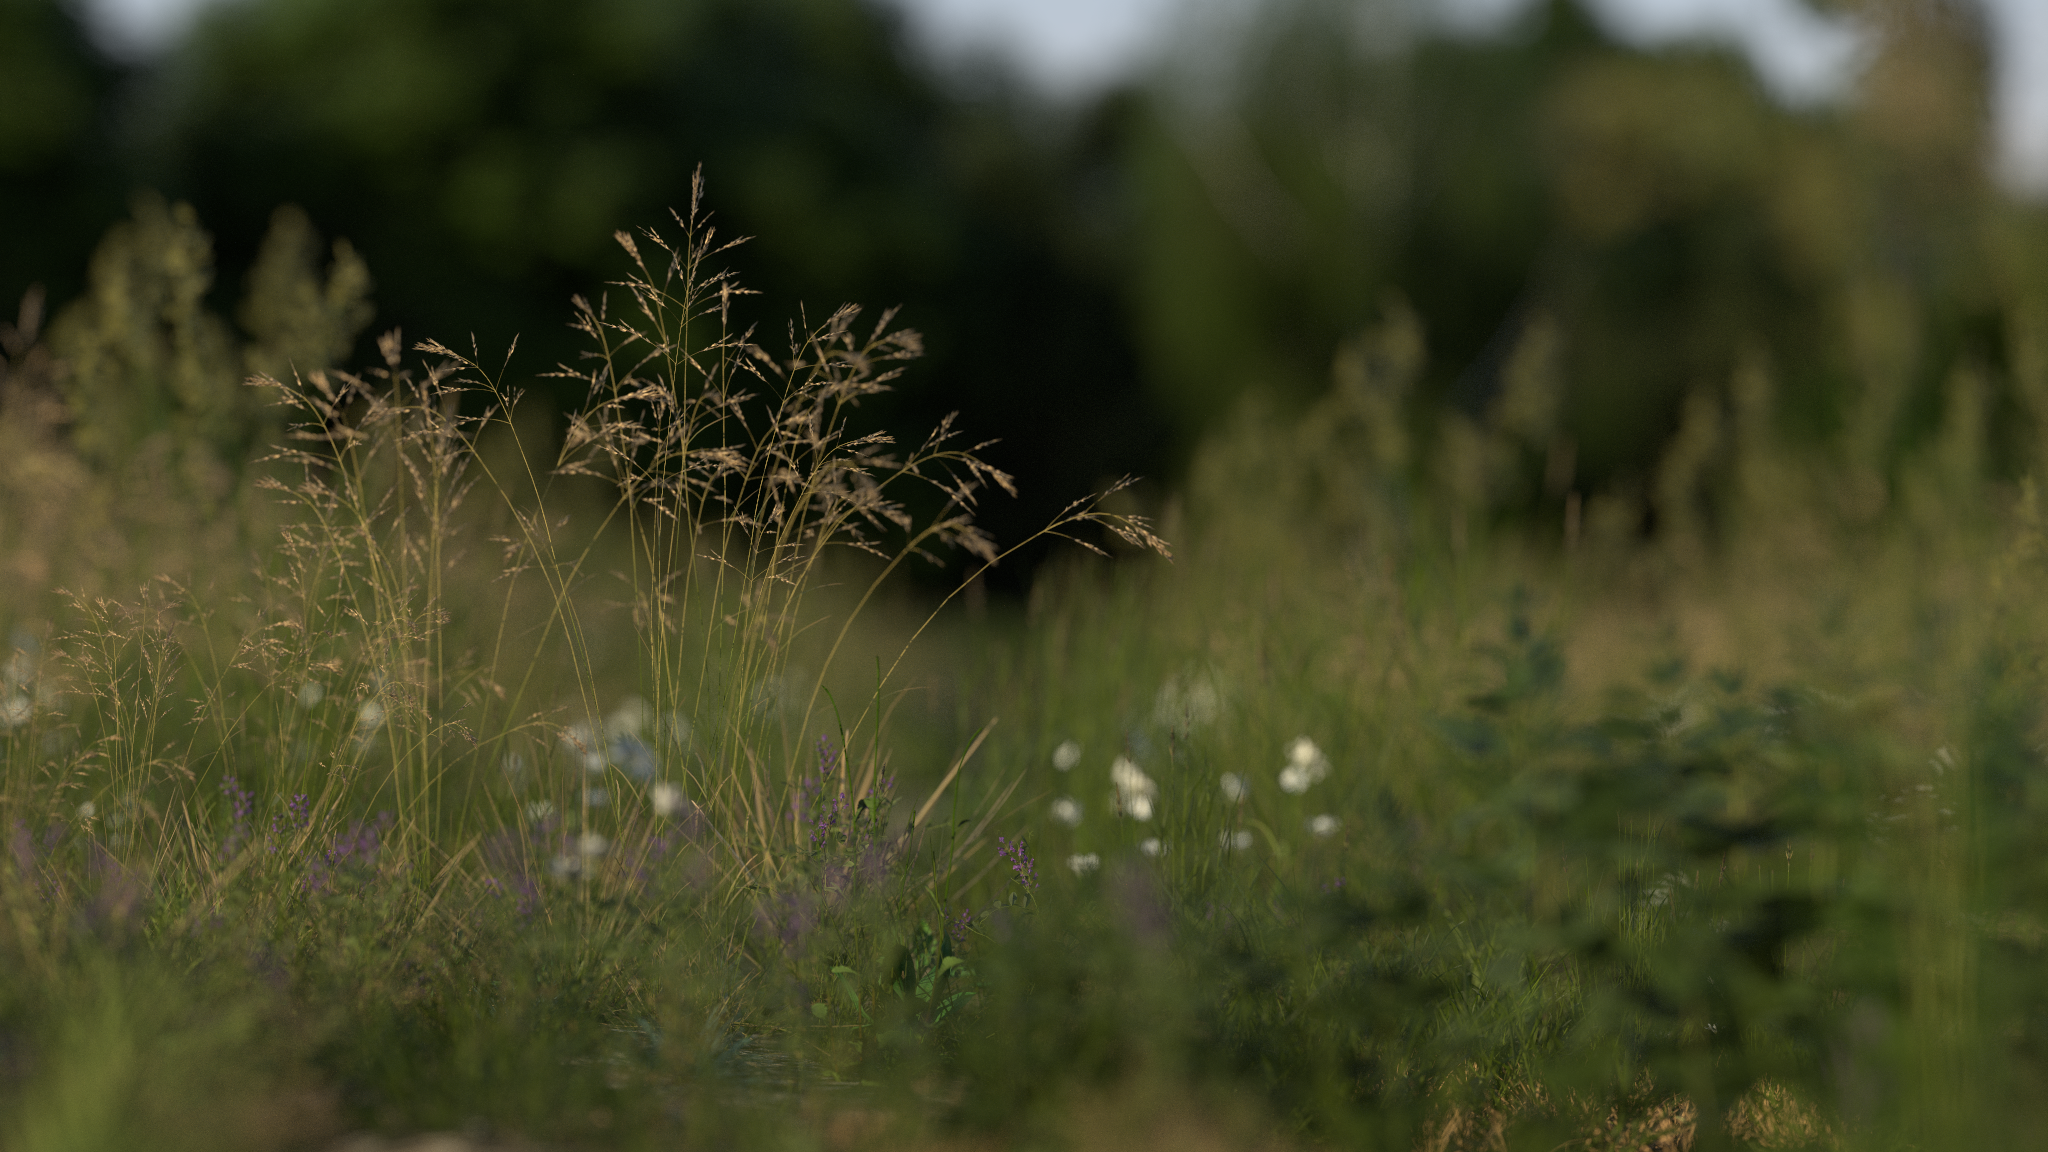
\includegraphics[height=\paperheight]{view-3.png}};
    \draw (current page.center) node [fill=yellow!80!green!40,fill opacity=0.1,text opacity=1,inner sep=1cm]
    {\centering\bfseries\sffamily\parbox[c][][t]{\paperwidth}{\color{white}\centering
    {\Large Physically Based Rendering: From Theory To Implementation}\\[25pt]
    {\fontsize{30pt}{15pt}\textrm{从理论到实现}}\\[15pt]
    {\fontsize{60pt}{15pt}\textrm{基于物理的渲染}}\\[25pt]
    {\fontsize{21pt}{15pt}第三版}\\[20pt]
    {\Large\begin{tabular}{rcl}原著 && Matt Pharr\\ && Wenzel Jakob\\ && Greg Humphreys\\ 翻译 && Kanition\end{tabular}}}};
\end{tikzpicture}
\vfill
\endgroup

%----------------------------------------------------------------------------------------
%	COPYRIGHT PAGE
%----------------------------------------------------------------------------------------

\newpage
~\vfill
\thispagestyle{empty}

\noindent \textbf{\LARGE 从理论到实现}\vspace{8pt}\\
\noindent \textbf{\Huge 基于物理的渲染}\vspace{8pt}\\
\noindent \textbf{\large 第三版}\vspace{8pt}\\
\noindent \textbf{\large 原著 \quad Matt Pharr, Wenzel Jakob \& Greg Humphreys}\vspace{5pt}\\
\noindent \textbf{\large 翻译 \quad Kanition}\vspace{16pt}\\

\noindent {\bfseries 英文原版}

\noindent Copyright \copyright\ 2004–2021 Matt Pharr, Wenzel Jakob, and Greg Humphreys

\noindent 官方网址:\url{http://www.pbr-book.org}

\noindent 许可证:CC BY-NC-SA 4.0\\

\noindent {\bfseries 本中译版}

\noindent Copyright \copyright\ 2021 Kanition

\noindent 更新网址:\url{https://github.com/kanition/pbrtbook}

\noindent 许可证:CC BY-NC-SA 4.0

    {\small(详见:\url{https://creativecommons.org/licenses/by-nc-sa/4.0})}\\

\noindent{\itshape
本中译版(以下简称“本书”)系译者(笔名 Kanition)自学英文经典书籍
《Physically Based Rendering: From Theory To Implementation》第三版时自行翻译而成。
使用本书及其源码须遵循相关许可证协议。

本书在翻译时并不完全遵照原书编排,而是根据我自己的学习情况作出了调整,
包括但不限于调整顺序、增删内容、修改内容。
例如扩展阅读和高阶内容部分往往超出了我的能力范围,这些内容可能会被省略;
再如有一些公式可能存在笔误,我会改写并注明。

此外,翻译并不追求从英语单词到中文字词的“一一映射”。
一些不涉及关键概念的词句可能会依据中文习惯作出修改,
只要表达了作者的核心原意即可。
因此发现英文原版词句和本书内容不完全对应是非常正常和常见的现象。

原书在线版本以网页形式呈现,可以方便地展开、折叠示例代码,但翻译制作成本书时则面临困难。
本书将视具体上下文情况对示例代码做补全、删减或修改。实践时请以原书所附代码为准。

本书由{\scshape \LaTeX} 编写而成,源码已经发布在上述网址,欢迎访问获取最新版。

{\sffamily{欢迎提出宝贵意见和建议。如果你发现本书存在错误,请一定要告诉我们!
讨论区:{\normalfont\url{https://github.com/kanition/pbrtbook/discussions}}}}
}

\newpage
\setcounter{page}{1}
\pagestyle{fancy}
{\Huge\bfseries 前言}\vspace{30pt}\\

渲染是计算机图形学的基础组成部分。
最抽象地说,渲染是把三维场景描述转换为图像的过程。
动画算法、几何建模、材质贴图和计算机图形学其他领域
都须经某些渲染过程来可视化其结果。
从电影到游戏等,渲染无处不在,它为创作、娱乐和可视化开辟了新的领域。

早期的渲染研究重点解决基本问题,例如从给定视点确定哪些物体是可见的。
随着这些问题找到高效解法以及图形学其他领域的持续发展使得场景描述更加丰富逼真,
现代渲染已涵盖了广泛内容,包括物理学、天体物理学、天文学、生物学、心理学、感知研究、理论和应用数学。
渲染的跨学科性是它如此引人的原因之一。

本书以文档化代码的形式提供了构建一个完整的渲染系统所需的一批现代渲染算法。
包括封面在内\sidenote{译者注:本书封面作了更换,但和原书封面是同一组渲染结果。},
本书几乎所有图像都由该软件渲染得到。
且生成这些图像的全部算法均有描述。
该pbrt系统按{\itshape 文学编程}的程序设计方法编写,
即把对系统的描述和实现源码结合在一起。
我们认为,用文学编程法介绍计算机图形学和计算机科学是非常合适的。
算法的一些微妙细节在实现之前往往很难弄清楚,
因此读实际代码更有利于充分理解它们。
我们相信,深入理解哪怕少量的算法也比跑马观花更能打牢进一步研究计算机图形学的基础。

除了阐明实践中如何实现算法外,交代其在完整简单软件系统中的上下文
同样有助于解决中型渲染系统的设计和实现问题。
渲染系统的基本抽象和接口设计对实现的优雅性和可扩展性有实质影响,
但本书不会讨论这类设计取舍。

pbrt和本书内容仅关注{\itshape 逼真渲染},
它可定义为这样的图像生成任务:和相机拍摄的照片难以区分,
或者人类看后被激发的响应与看到实际场景时一致。
我们有许多理由关注逼真感。
逼真图像对电影特效工业至关重要,
因为计算机生成的图像经常必须和真实世界的镜头无缝结合。
娱乐应用中所有图像都是合成的,
逼真感是让观察者忘记所见场景并不实际存在的有效手段。
最后,逼真感为衡量渲染系统输出质量提供了定义合理的指标。\\

\noindent{\LARGE\bfseries 读者}

本书主要面向三类读者。
第一类是学习计算机图形学课程的研究生或高年级本科生。
本书假定读者拥有大学入门级计算机图形学知识,
只会回顾一些关键概念,例如基本向量几何和变换。
对于没有编写过上万行源码程序的学生,
文学编程风格更能降低学习难度。
为了让读者领会为何要这样构建系统,
我们特别注意解释关键接口和抽象背后的设计考量。

第二类读者是计算机图形学研究人员。
本书为研究人员全面介绍了该领域,
pbrt源码提供了可用的构建基础(至少可使用一部分源码)。
对于其他领域的读者,
我们认为对透彻理解渲染也有助于了解相关背景。

最后一类读者是工业界软件开发者。
尽管这些读者可能很熟悉本书许多内容,
但阅读文学风格的算法解释也许能获取新的角度。
pbrt涵盖了大量高级或艰深算法的实现和技术,
例如细分曲面、蒙特卡洛采样算法、双向路径追踪、Metropolis采样和次表面散射;
经验丰富的渲染从业者应该会很感兴趣。
我们希望能激发这些读者去钻研一个完整而典型的渲染系统的兴趣。\\

\noindent{\LARGE\bfseries 概述和目标}

pbrt基于{\itshape 光线追踪}算法。
光线追踪是一项优雅的技术,起源于镜片制造。
19世纪Carl Friedrich Gau{\ss}就用透镜手动追踪光线。
计算机上的光线追踪算法跟随无穷小的光线穿过场景直到与曲面相交。
它给出了从特定位置和方向寻找第一个可见物体的简单方法,
这是许多渲染算法的基础。

pbrt的设计和实现贯彻了三个目标:{\itshape 完整性}、{\itshape 解说性}和基于{\itshape 物理性}。

完整性指系统不应缺少高质量商业渲染系统的关键功能。
这意味着要彻底解决重要的实际问题,
例如抗锯齿、稳定性、数值精度以及高效渲染复杂场景的能力。
在设计系统时一开始就应考虑到这些,
因为它们会对系统所有组件产生微妙影响,
且在实现后期阶段很难再改装到系统中。

第二个目标意味着我们着眼于可读性和清晰度,
精心选用算法、数据结构和渲染技术。
因为比起其他渲染系统,我们的实现要接受更多读者的检验,
所以我们尽力选择已知的最优算法并将其实现。
这个目标也要求系统要小到一个人能完全理解的程度。
我们用可扩展的架构实现了pbrt,
即系统核心采用精心设计的抽象基类,
且这些基类尽量实现足够多特定功能。
这样读者不用理解所有特定细节就能明白系统的基本结构。
这更易于钻研感兴趣的部分并跳过其他内容,
且不影响对系统整体配合的把握。

完整性和解说性目标之间是存在矛盾的。
涵盖所有可能有用的技术不仅让本书过于冗长,
而且对于大多数读者而言也太复杂。
针对万一pbrt缺少某项有用功能的情况,
我们尽量使架构便于增添功能而不用改变系统整体设计。

基于物理的渲染的基础是物理定律及其数学表达式。
pbrt的设计对所计算的量和实现的算法使用正确的物理单位。
这样配置后,pbrt能计算出{\itshape 物理正确}的图像;
它们像在真实世界场景中那样准确反映光照。
这样的好处是它为程序正确性提供了具体标准:
对于预期结果可用闭式解计算的简单场景,
如果pbrt没有算出相同结果,我们就能知道实现一定有bug。
类似地,如果pbrt中基于物理光照的不同算法对同一场景给出了不同结果,
或者pbrt所得结果和另一个基于物理的渲染器不一致,
则它们中必有一个出错了。
最后,我们认为基于物理的渲染方法是有价值的,因为它是严格的。
当不清楚特定计算该如何执行时,物理学会给出确保一致的答案。

效率的优先度低于以上三个目标。
既然渲染系统生成一张图像通常要花费数分钟或小时,
效率显然是很重要的。
然而我们主要关注{\itshape 算法}层面的效率而非底层代码优化。
尽管系统中计算量集中的部分已尽力做了优化,
但有时明显而微小的优化会让位于清晰的代码组织。

在介绍pbrt和讨论其实现时,
我们希望传授多年来渲染研究和开发的经验教训。
编写好一个渲染器比串接一堆快速算法更需要付出;
让系统既灵活又稳定是项困难的任务。
随着增添越来越多的几何体或光源,
或者其他复杂维度上升,
系统的性能将逐渐下降。
严谨处理数值稳定性、
算法不浪费浮点精度也至关重要。

开发出解决所有这些问题的系统大有益处——
编写新的渲染器或向已有渲染器添加新功能并用它创作出以往无法生成的图片是多么地快乐。
我们编写本书最基本的目标就是给广大读者这样的机会。
我们鼓励读者在阅读本书时使用该系统渲染pbrt发行的示例场景。
每章末的习题会要求修改系统以加深对内部工作原理的理解,
或者完成添加新功能等更复杂的工程。

本书官网为\url{www.pbrt.org},
可从该站获取pbrt最新版源码。
我们也会发布勘误、修复bug、新增渲染场景和补充材料。
遇到网站尚未列出的pbrt中的任何bug或行文错误
均发送到邮箱\href{mailto:bugs@pbrt.org}{\url{bugs@pbrt.org}}。
我们非常重视您的反馈\sidenote{译者注:我也欢迎您的反馈!详见扉页更新网址。}!\\

\noindent{\LARGE\bfseries 第一版和第二版的区别}

{\itshape 详见英文原版}\\

\noindent{\LARGE\bfseries 第二版和第三版的区别}

{\itshape 详见英文原版}\\

\noindent{\LARGE\bfseries 致谢}

{\itshape 详见英文原版}\\

\noindent{\LARGE\bfseries 出版}

{\itshape 详见英文原版}\\

\noindent{\LARGE\bfseries 场景和模型}

{\itshape 详见英文原版}\\

\noindent{\LARGE\bfseries 关于封面}

{\itshape 详见英文原版}\\

\noindent{\LARGE\bfseries 扩展阅读}

Donald Knuth的论文《Literate Programming》\citep{10.1093/comjnl/27.2.97}
描述了文学编程背后的主要思想以及他的网络编程环境。
开创性的\TeX 排版系统是用网络写成的并出版了一系列书籍\citep{10.5555/536126,10.5555/536123}。
最近,Knuth在《The Stanford GraphBase》\citep{10.1145/164984}中
以文学格式出版了图表算法集。
这些程序读起来很有趣,各个算法也展示得很好。
网站\url{www.literateprogramming.com}指向了许多关于文学编程的论文、程序以及大量系统;
自Knuth最初提出该思想以来,文学编程已经进行了许多改进。


我们所知的其他出版成书的文学程序只有对lcc编译器的实现——
由Christopher Fraser和David Hanson编写
并出版的《A Retargetable C Compiler: Design and Implementation》\citep{10.5555/555424},
以及Martin Ruckert关于MP3音频格式的书《Understanding MP3》\citep{10.5555/1036653}。


\newpage
{\Huge\bfseries 在线版序言}\vspace{30pt}\\

2004年发行的第一版《基于物理的渲染》只有纸质书。
2010年第二版新增了Kindle版,但不幸的是
所有交叉引用和索引都在转换中丢失了。
终于,2016年发布的第三版转换出了良好的Kindle版和PDF版。
尽管电子版有所改进,但我们觉得它还远称不上完美。

文学编程是《基于物理的渲染》的核心。
它是Donald Knuth提出的一种软件编写方法,
比起在计算机上把源码转换为可执行指令,
它更重视人类阅读源码时的直观性。
文学编程将复杂程序分解为便于理解的片段,
并提供多种方式对其交叉引用,以帮助理解每个片段的内容。

对于纸上的文学编程,每页都有丰富的辅助信息并编有定向页码。
边栏有索引指向当前页所用标识符对应的代码定义所在的页码,
并且每个代码段都有表示其它部分定义所在页码和被引用的页码。

这种格式很有效,但页码绕得烦人。
而且翻书找页也很麻烦。
我们想到,如果把电子设备——台式机、笔记本、平板甚至手机——
作为本书内容的主要交付工具,我们会获得怎样的阅读体验?
没有页码了,取而代之的是超链接,直接把读者引向目标且容易返回原处。

改善的不仅只有导航:
现代显示器比打印纸有好得多的色彩保真度和动态范围,
结合计算机使用还能与书中图示交互。
对于通篇在讲图像与三维世界的书籍而言这是极大的优点。

2018年夏季,我们获取到出版商的授权;
我们非常感谢他们慷慨归还版权。
这样我们就能自由决定是否尝试以这种新形式呈现本书内容。
我们的答案是肯定的。
遭受一个月的黑客攻击后,
我们实现了一个系统,
把本书从以前编写时所用的标记语言转换为HTML。
你现在读的就是它\sidenote{译者注:原作者可能没料到有人又把它翻译回PDF了。}。

本书在线版与第三版《基于物理的渲染》很接近。
我们只作了以下修改:
\begin{itemize}
    \item 更新一些插图所用的渲染图像,
    \item 为图像查看增加交互,
    \item 重画所有插图,
    \item 把比较同一场景的不同渲染结果的多幅图像合并为一幅图像,
    \item 合并读者反馈的勘误。
\end{itemize}

前两点还需要说明一下。关于更新图像:
纸质书的一大挑战是确保诸如蒙特卡洛噪声等图像痕迹在页面上可见。
我们担心印刷会引入多余的模糊,
也担心成书过程中有好心人帮倒忙给图像降噪使其看起来更清晰。
因此我们用最近邻滤波器放大了本应展现差错的图像,
使这些差错能在印刷过程中保留下来。

现在这个担心是多余的了。
很高兴能重新渲染这些图像,
连一个像素大小的差错都能保留了。

第二点修改标志着我们朝交互式内容探究迈出了第一步:
在网页浏览器中,可以细究渲染图像的细节和区别,
这是纸质书做不到的。
在线版大多数渲染图像都能放大、全屏查看以及和其他图像比较。
它们都有此图标
\sidenote{译者注:在线版是一片雪花图案。
    不过PDF没法实现网页端那么强大的交互功能,
    所以阅读本书时就无视它吧。}:*。
将鼠标悬停在该图标上可获取相关操作的详细信息。\\

\noindent{\LARGE\bfseries 路线图}

本书计划大致每年发布一次更新
\sidenote{译者注:本书在翻译时已经发布第四版代码了,但还未在线发布书籍。}。
尽管在线版比纸质版更容易快速更新,
我们还是认为适当的更新速度有利于对下次发布做严谨的检查和编辑。

除了扩展pbrt功能跟进最新研究,
我们还计划为新版增加更多交互元素。
Str{\"o}m、{\AA}str{\"o}m和Akenine-M{\"o}ller
编写的《\citetitle{4b212a02-105c-42a2-ad5c-91c16a06e815}》\footnote{\citeurl{4b212a02-105c-42a2-ad5c-91c16a06e815}}
一书展现了这种媒体的无限可能。

我们会在线保留本书的早前版本,URL均和首发时保持一致;
新版会放在单独的目录中。
因此链接到此处的内容是安全的,不必担心未来断链
\sidenote{译者注:本中译版不作此承诺。}。\\

\noindent{\LARGE\bfseries 报告错误}

{\itshape 详见英文原版}\\

\noindent{\LARGE\bfseries 致谢}

{\itshape 详见英文原版}\\

\noindent{\LARGE\bfseries 许可证}

{\itshape 详见英文原版}

%----------------------------------------------------------------------------------------
%	TABLE OF CONTENTS
%----------------------------------------------------------------------------------------
\renewcommand{\contentsname}{目录}

%\usechapterimagefalse % If you don't want to include a chapter image, use this to toggle images off - it can be enabled later with \usechapterimagetrue

\chapterimage{Pictures/measure-one180-cut1260.png} % Table of contents heading image

\pagestyle{empty} % Disable headers and footers for the following pages

\tableofcontents % Print the table of contents itself

\cleardoublepage % Forces the first chapter to start on an odd page so it's on the right side of the book

\pagestyle{fancy} % Enable headers and footers again

%----------------------------------------------------------------------------------------
%	PART
%----------------------------------------------------------------------------------------

\part{绪论}

%----------------------------------------------------------------------------------------
%	CHAPTER 1
%----------------------------------------------------------------------------------------

\chapterimage{Pictures/chap01/nightsnow-cut1368.png}

\chapter{绪论}\label{chap:绪论}

\keyindex{渲染}{rendering}{render渲染}是
由3D\keyindex{场景}{scene}{}描述生成图像的过程。
显然,这是一项十分庞大的任务,
有许多解决方案。\keyindex{基于物理的}{physically based}{physics物理}
的技术采用模拟现实,
即运用物理学规律对光与物质的\keyindex{相互作用}{interaction}{}建模。
尽管基于物理的方法是实现渲染最容易想到的办法,
但它最近十年才在实践中得到广泛运用。
本章末的\refsec{基于物理的渲染简史}
将给出基于物理的渲染的简史
以及它近来在电影\keyindex{离线渲染}{offline rendering}{render渲染}和
游戏\keyindex{交互式渲染}{interactive rendering}{render渲染}方面的应用。

本书将介绍\emph{pbrt}这一基于\keyindex{光线追踪}{ray-tracing}{ray光线}算法的基于物理的渲染系统。
大多数计算机\keyindex{图形学}{graphics}{}书籍都主讲算法和理论,
偶尔附上一小段代码。
相反,本书将理论和一个功能齐全的渲染系统的完整实现结合起来。
系统的完整代码\footnote{\url{https://github.com/mmp/pbrt-v3}}
可在BSD许可证下获取。
在pbrt网站\url{https://pbrt.org}还可获取示例场景、渲染数据等更多信息。

\section{文学编程}\label{sec:文学编程}

在编写\TeX 排版系统时,Donald Knuth新提出一种简单但具有革命性的
编程方法论:\emph{程序应该写得更便于人类使用而不是更便于计算机理解}。
他将其称作\keyindex{文学编程}{literate programming}{}。
本书(包括本章)就是一个长长的文学程序。
这意味着在阅读本书的过程中,
你会读到pbrt渲染系统的\emph{完整}实现,
而不仅仅是高层叙述。

文学程序是由\keyindex{元语言}{metalanguage}{}
写成的,该语言把文档格式语言(例如\TeX 或HTML)
和编程语言(例如C++)结合起来。
两套分离的系统会这样处理程序:\keyindex{编排器}{weaver}{literate programming文学编程}
把文学程序转换成适合排版的文档,\keyindex{整合器}{tangler}{literate programming文学编程}
则生成可供编译的源码\sidenote{译者注:我不太确定编排器和整合器的翻译是否合适。}。
虽然我们的文学编程系统是自研的,
但很大程度上受到了Norman Ramsey的\emph{noweb}系统的影响。

文学编程元语言提供了两个重要功能。
第一个是把行文与源码结合起来。
这个功能让程序的说明和实际源码一样重要,
促使设计和文档做得更细致。
第二个是提供了与输入编译器的顺序完全不同的向读者展示程序代码的机制。
因此可以按逻辑顺序阐述程序。
每一段具有名称的代码块叫作\keyindex{代码片}{fragment}{},
每个代码片可以通过名称引用其他代码片。

例如,考虑一个负责初始化程序全部全局变量的函数
\footnote{本节的代码仅用作示例,不属于pbrt的一部分。}
{\ttfamily InitGlobals()}:
\begin{lstlisting}
void InitGlobals() {
    nMarbles = 25.7;
    shoeSize = 13;
    dielectric = true;
}
\end{lstlisting}

这个函数虽然很简短,但很难在没有任何上下文的情况下搞懂它。
比如为什么变量{\ttfamily nMarbles}采用浮点值?
刚看这段代码时,
就得在整个程序里寻找每个变量是在哪里声明的、怎么用的,
好弄清它的目的和合法值的含义。
尽管这样的系统结构对编译器来说没问题,
但人类阅读者更愿意看到
每个变量的初始化代码是分开呈现的,
而且最好紧挨着实际声明和使用这些变量的代码。

在文学程序中,可以把\refvar{InitGlobals}{()}写成这样:
\begin{lstlisting}
`\initcode{Function Definitions}{=}`
void `\initvar{InitGlobals}{()}` {
    `\refcode{Initialize Global Variables}{\dag}`
}
\end{lstlisting}

这就定义了称作\refcode{Function Definitions}{}的代码片,
包含了函数\refvar{InitGlobals}{()}的定义。
函数\refvar{InitGlobals}{()}自己又引用了另一
代码片\refcode{Initialize Global Variables}{}。
因为初始化的代码片还没有定义,
所以我们只知道这个函数可能会对全局变量赋值
(然而我们可以通过单击右边的加号\sidenote{译者注:本中译版改为直接点击代码片名称。}向前跳转;
这样可以展开代码片最终全部的代码)。

现在有了代码片名称仅仅是有了正确的抽象层级,
因为还没有声明过任何变量。
之后在程序某处引入全局变量{\ttfamily shoeSize}时,
我们可以这样写:
\begin{lstlisting}
    `\initcode{Initialize Global Variables}{=}\initnext{InitializeGlobalVariables}`
    shoeSize = 13;
\end{lstlisting}

这里我们开始定义\refcode{Initialize Global Variables}{}的内容了。
当文学程序整合成待编译的源码时,
文学编程系统会把代码{\ttfamily shoeSize = 13;}
替换到函数\refvar{InitGlobals}{()}的定义内。
等号后的符号{\codecolor $\downarrow$}表示后续还有代码添加到该代码片。
点击它即可跳转到下一处。

后文我们也许又定义了另一个全局变量{\ttfamily dielectric},
可以这样把它的初始化添到代码片之后:
\begin{lstlisting}
    `\refcode{Initialize Global Variables}{+=}\lastcode{InitializeGlobalVariables}`
    dielectric = true;
\end{lstlisting}

代码片名后的符号{\codecolor +=}表示我们之前已经定义过该代码片了。
此外符号{\codecolor $\uparrow$}回链到
之前\refcode{Initialize Global Variables}{}添加代码的地方。

当整合时,这三个代码片转换为代码:
\begin{lstlisting}
void InitGlobals() {
    `\hypertarget{code:Initialize Global Variables}{\color[RGB]{115,48,11}\scriptsize\rmfamily// Initialize Global Variables}`
    shoeSize = 13;
    dielectric = true;
}
\end{lstlisting}

这样,我们可以把复杂函数分解为逻辑不同的部分,使之更容易理解。
例如我们可以这样把一个复杂函数写作一系列代码片:
\begin{lstlisting}
`\refcode{Function Definitions}{+=}`
void `\initvar{complexFunc}{(int x, int y, double *values)}` {
    `\refcode{Check validity of arguments}{}`
    if (x < y) {
        `\refcode{Swap parameter values}{}`
    }
    `\refcode{Do precomputation before loop}{}`
    `\refcode{Loop through and update \textbackslash mono\{values\} array}{}`
}
\end{lstlisting}

同样,编译时\refvar{complexFunc}{()}内每段代码片的内容都内联展开。
在文档中,我们可以依次介绍每个代码片的实现。
这种分解让我们每次只展示一小段代码,使之更易于理解。
这种编程风格的另一优点是,通过把函数分解为逻辑片,
每片有了单一且明确的目的,可以独立编写、验证、阅读。
一般我们尽量让每段代码片少于10行。

在某种意义上,文学编程系统只是个增强了的宏替换包,
完成重排程序源码的任务。
这变化看似微不足道,但事实上文学编程和其他软件构建系统方法迥然不同。



\section{逼真渲染和光线追踪算法}\label{sec:逼真渲染和光线追踪算法}

逼真渲染的目标是创建3D场景的图像且与同一场景的照片难以区分。
在我们介绍渲染流程之前要重点理解的是,
此处的{\itshape 难以区分}一词不是精确说法,
因为它涉及人类观察者,
不同观察者对同一图像的感知可能是不同的。
尽管本书会涉及少量感知问题,
但明确给出观察者的精确特性是非常困难且远未解决的问题。
绝大多数时候,我们都对针对光及其与物质相互作用的物理仿真感到满意,
并以我们对显示技术的理解尽可能向观察者展示最好的图像。

几乎所有逼真渲染系统都基于光线追踪算法。
光线追踪算法其实很简单;
它跟随光线\sidenote{译者注:原文a ray of light。
    此外会按个人理解把ray译作“光线”或“射线”,把light译作“光”或“光线”。}路径
穿过场景与环境中的物体相互作用并反射。
虽然编写光线追踪器的方法有很多,
但所有这些系统都必须模拟至少一项以下对象和现象:
\begin{itemize}
    \item \keyindex{相机}{cameras}{camera相机}: 相机模型决定了从哪里、怎样观察场景,
          包括场景的图像是怎样记录到传感器上的。
          许多渲染系统从相机处开始生成视线并追踪到场景中。
    \item \keyindex{光线-物体交点}{ray–object intersections}{ray光线}: 此外,我们需要确定
          交点处物体的特定属性,例如表面法线或材质。
          多数光线追踪器都有测试光线与多个物体相交的功能,
          典型的例如沿光线返回最近交点。
    \item \keyindex{光源}{light sources}{light光}: 没有光,渲染场景就没有意义。
          光线追踪器必须对整个场景的光分布建模,
          不仅包括灯光自身的位置,还包括它们向整个场景发散能量的方式。
    \item \keyindex{可见性}{visibility}{}:为了知道给定光是否在表面上一点积累能量,
          必须确认从该点到光源是否存在一条不中断的路径。
          幸运的是,在光线追踪器中这个问题很容易回答,
          因为我们可以构造从表面到光源\sidenote{译者注:原文为light,我按个人理解译作“光源”。}的射线,
          寻找最近的光线-物体交点,
          并比较交点距离和光源距离。
    \item \keyindex{表面散射}{surface scattering}{}:每个物体都必须提供外观描述,
          包括光如何与物体表面相互作用等信息,
          以及再辐射\sidenote{译者注:原文reradiated。}(或散射\sidenote{译者注:原文scattered。})光的性质。
          表面散射模型是典型的参数化模型,
          因此可以模拟各种外观。
    \item \keyindex{间接光传输}{indirect light transport}{light光}\sidenote{译者注:这里把transport译作“传输”是为了
              与下一段propagation译作“传播”区分开,但个人理解似乎就是“传播”的意思。}:因为
          光在一个物体上反射或折射后可能遇到另一个物体,
          所以通常有必要追踪从表面发出的额外光线来捕捉这种效应。
    \item \keyindex{光线传播}{ray propagation}{ray光线}:我们需要知道光在空间中沿光线传播时发生了什么。
          如果渲染真空中的场景,则光能量沿光线保持恒定。
          真正的真空虽然在地球上是罕见的,
          但对许多环境而言是合理的近似。
          更多复杂模型可用于追踪穿过雾、烟、大气等的光线。
\end{itemize}

本节我们将简要讨论以上每个仿真任务。
后续章节我们会展示pbrt底层仿真组件的高级接口,
了解贯穿主渲染循环的单个光线处理过程。
我们还会介绍基于Turner Whitted的
原始光线追踪算法的表面散射模型实现。

\subsection{相机}\label{sub:相机}

几乎每个人都用过\keyindex{相机}{camera}{},熟悉它的基本功能:
你表达记下世界的一张图像的愿望(通常是按按钮或点击屏幕),
然后图像就被记录到\keyindex{胶片}{film}{}或电子传感器上。
最简单的拍照设备之一称作\keyindex{针孔相机}{pinhole camera}{camera相机}。
针孔相机由一端打有小孔的遮光盒组成(\reffig{1.1})。
当孔未被遮挡时,光射进孔落到固定在盒子另一端的相纸上。
虽然它很简单,但这种相机至今仍在使用,常用于艺术目的。
要在胶片上获得足够的光以形成图像需要非常长的曝光时间。
\begin{figure}[h]
    \centering%LaTeX with PSTricks extensions
%%Creator: Inkscape 1.0.1 (3bc2e813f5, 2020-09-07)
%%Please note this file requires PSTricks extensions
\psset{xunit=.5pt,yunit=.5pt,runit=.5pt}
\begin{pspicture}(719.89001465,221.22999573)
{
\newrgbcolor{curcolor}{0 0 0}
\pscustom[linewidth=1,linecolor=curcolor]
{
\newpath
\moveto(180.38,220.31999573)
\lineto(54.38,140.19999573)
\lineto(54.38,1.18999573)
\lineto(180.38,81.30999573)
\closepath
}
}
{
\newrgbcolor{curcolor}{0 0 0}
\pscustom[linewidth=1,linecolor=curcolor]
{
\newpath
\moveto(393.38,220.31999573)
\lineto(267.38,140.19999573)
\lineto(267.38,1.18999573)
\lineto(393.38,81.30999573)
\closepath
}
}
{
\newrgbcolor{curcolor}{0 0 0}
\pscustom[linewidth=1,linecolor=curcolor]
{
\newpath
\moveto(180.02000427,220.5699957)
\lineto(393.23999023,220.5699957)
}
}
{
\newrgbcolor{curcolor}{0.72156864 0.70980394 0.70980394}
\pscustom[linestyle=none,fillstyle=solid,fillcolor=curcolor]
{
\newpath
\moveto(153.14,161.25999573)
\lineto(96.9,125.49999573)
\lineto(96.9,63.44999573)
\lineto(153.14,99.20999573)
\closepath
}
}
{
\newrgbcolor{curcolor}{0 0 0}
\pscustom[linewidth=1,linecolor=curcolor]
{
\newpath
\moveto(153.14,161.25999573)
\lineto(96.9,125.49999573)
\lineto(96.9,63.44999573)
\lineto(153.14,99.20999573)
\closepath
}
}
{
\newrgbcolor{curcolor}{0 0 0}
\pscustom[linewidth=1,linecolor=curcolor]
{
\newpath
\moveto(53.95000076,140.56999207)
\lineto(266.80999756,140.56999207)
}
}
{
\newrgbcolor{curcolor}{0 0 0}
\pscustom[linewidth=1,linecolor=curcolor]
{
\newpath
\moveto(180.02000427,82)
\lineto(393.58999634,82)
}
}
{
\newrgbcolor{curcolor}{0 0 0}
\pscustom[linewidth=1,linecolor=curcolor]
{
\newpath
\moveto(54.31000137,0.5)
\lineto(267.16000366,0.5)
}
}
{
\newrgbcolor{curcolor}{0 0 0}
\pscustom[linewidth=1,linecolor=curcolor]
{
\newpath
\moveto(339.7301427,119.158401)
\curveto(341.5742157,118.06695026)(341.46601021,114.47358161)(339.48845898,111.1323875)
\curveto(337.51090776,107.79119338)(334.41286921,105.96741604)(332.56879621,107.05886679)
\curveto(330.72472322,108.15031754)(330.8329287,111.74368618)(332.81047993,115.0848803)
\curveto(334.78803116,118.42607441)(337.88606971,120.24985175)(339.7301427,119.158401)
\closepath
}
}
{
\newrgbcolor{curcolor}{0 0 0}
\pscustom[linewidth=1,linecolor=curcolor]
{
\newpath
\moveto(576.36,162.31999573)
\lineto(520.12,126.55999573)
\lineto(520.12,64.50999573)
\lineto(576.36,100.26999573)
\closepath
}
}
{
\newrgbcolor{curcolor}{0 0 0}
\pscustom[linewidth=1,linecolor=curcolor]
{
\newpath
\moveto(153.71000671,161.95999527)
\lineto(631.82000732,33.97999573)
}
}
{
\newrgbcolor{curcolor}{0 0 0}
\pscustom[linewidth=1,linecolor=curcolor]
{
\newpath
\moveto(97.04000092,125.74999237)
\lineto(617.29998779,98.77999878)
}
}
{
\newrgbcolor{curcolor}{0 0 0}
\pscustom[linewidth=1,linecolor=curcolor]
{
\newpath
\moveto(96.43000031,63.16999817)
\lineto(673.23999023,182.71999741)
}
}
{
\newrgbcolor{curcolor}{0 0 0}
\pscustom[linewidth=1,linecolor=curcolor]
{
\newpath
\moveto(152.83999634,99.34999847)
\lineto(622.55999756,133.60999298)
}
}
{
\newrgbcolor{curcolor}{0 0 0}
\pscustom[linewidth=0.5,linecolor=curcolor]
{
\newpath
\moveto(379.01000977,47.37998962)
\lineto(338.20001221,103.22999573)
}
}
{
\newrgbcolor{curcolor}{0 0 0}
\pscustom[linewidth=0.5,linecolor=curcolor]
{
\newpath
\moveto(47.15000153,86.3999939)
\lineto(91.18000031,90.69999695)
}
}
{
\newrgbcolor{curcolor}{0 0 0}
\pscustom[linestyle=none,fillstyle=solid,fillcolor=curcolor]
{
\newpath
\moveto(369.586782,39.9484801)
\lineto(369.586782,41.0844801)
\lineto(366.242782,41.0844801)
\curveto(366.498782,41.5644801)(366.722782,42.0764801)(366.898782,42.5724801)
\lineto(365.842782,42.8924801)
\curveto(365.314782,41.4204801)(364.386782,39.9804801)(363.378782,39.0524801)
\curveto(363.570782,38.7964801)(363.890782,38.1884801)(363.986782,37.9484801)
\curveto(364.546782,38.5084801)(365.090782,39.1804801)(365.602782,39.9484801)
\closepath
\moveto(367.378782,30.4284801)
\lineto(367.378782,33.9644801)
\lineto(369.506782,33.9644801)
\lineto(369.506782,35.0524801)
\lineto(367.378782,35.0524801)
\lineto(367.378782,37.2124801)
\lineto(369.186782,37.2124801)
\lineto(369.186782,38.2844801)
\lineto(364.594782,38.2844801)
\lineto(364.594782,37.2124801)
\lineto(366.242782,37.2124801)
\lineto(366.242782,35.0524801)
\lineto(363.842782,35.0524801)
\lineto(363.842782,33.9644801)
\lineto(366.242782,33.9644801)
\lineto(366.242782,30.6524801)
\curveto(366.242782,29.9964801)(365.794782,29.6284801)(365.506782,29.4524801)
\curveto(365.714782,29.1964801)(365.970782,28.7004801)(366.066782,28.4124801)
\curveto(366.354782,28.6844801)(366.802782,28.9244801)(369.922782,30.5564801)
\curveto(369.842782,30.7964801)(369.746782,31.2604801)(369.714782,31.5804801)
\closepath
\moveto(378.034782,37.5964801)
\lineto(374.594782,37.5964801)
\lineto(374.594782,42.7964801)
\lineto(373.394782,42.7964801)
\lineto(373.394782,37.5964801)
\lineto(369.666782,37.5964801)
\lineto(369.666782,36.4284801)
\lineto(373.394782,36.4284801)
\lineto(373.394782,28.3324801)
\lineto(374.594782,28.3324801)
\lineto(374.594782,36.4284801)
\lineto(378.034782,36.4284801)
\closepath
}
}
{
\newrgbcolor{curcolor}{0 0 0}
\pscustom[linestyle=none,fillstyle=solid,fillcolor=curcolor]
{
\newpath
\moveto(386.62675148,42.0444801)
\lineto(386.38675148,41.9644801)
\lineto(379.77875148,41.9644801)
\lineto(379.77875148,40.8604801)
\lineto(385.47475148,40.8604801)
\curveto(384.77075148,40.0284801)(383.82675148,39.1324801)(382.97875148,38.5564801)
\lineto(382.97875148,35.4844801)
\curveto(381.61875148,35.1324801)(380.37075148,34.8124801)(379.42675148,34.5724801)
\lineto(379.68275148,33.3884801)
\lineto(382.97875148,34.3004801)
\lineto(382.97875148,29.8204801)
\curveto(382.97875148,29.5804801)(382.89875148,29.5164801)(382.64275148,29.5004801)
\curveto(382.41875148,29.5004801)(381.60275148,29.5004801)(380.70675148,29.5324801)
\curveto(380.89875148,29.1804801)(381.04275148,28.6684801)(381.09075148,28.3324801)
\curveto(382.25875148,28.3164801)(383.04275148,28.3484801)(383.52275148,28.5404801)
\curveto(383.98675148,28.7484801)(384.13075148,29.0844801)(384.13075148,29.8044801)
\lineto(384.13075148,34.6044801)
\lineto(387.37875148,35.5004801)
\lineto(387.21875148,36.6204801)
\curveto(386.19475148,36.3324801)(385.15475148,36.0444801)(384.13075148,35.7884801)
\lineto(384.13075148,38.0764801)
\curveto(385.29875148,38.9724801)(386.59475148,40.2684801)(387.42675148,41.4524801)
\closepath
\moveto(390.37075148,29.5484801)
\curveto(389.76275148,29.5484801)(389.63475148,29.6924801)(389.63475148,30.5084801)
\lineto(389.63475148,42.5564801)
\lineto(388.46675148,42.5564801)
\lineto(388.46675148,30.5404801)
\curveto(388.46675148,28.9244801)(388.83475148,28.4764801)(390.22675148,28.4764801)
\lineto(392.46675148,28.4764801)
\curveto(393.84275148,28.4764801)(394.14675148,29.3724801)(394.27475148,32.0124801)
\curveto(393.95475148,32.0924801)(393.49075148,32.3004801)(393.20275148,32.5404801)
\curveto(393.12275148,30.1404801)(393.02675148,29.5484801)(392.38675148,29.5484801)
\closepath
}
}
{
\newrgbcolor{curcolor}{0 0 0}
\pscustom[linestyle=none,fillstyle=solid,fillcolor=curcolor]
{
\newpath
\moveto(24.961985,91.8927451)
\lineto(20.801985,91.8927451)
\lineto(21.873985,92.3407451)
\curveto(21.665985,92.9167451)(21.153985,93.7167451)(20.641985,94.3087451)
\lineto(19.585985,93.8927451)
\curveto(20.081985,93.2847451)(20.545985,92.4527451)(20.769985,91.8927451)
\lineto(16.721985,91.8927451)
\lineto(16.721985,90.7887451)
\lineto(24.961985,90.7887451)
\closepath
\moveto(21.761985,89.8447451)
\curveto(22.769985,88.8047451)(23.953985,87.3487451)(24.449985,86.3887451)
\lineto(25.345985,87.1087451)
\curveto(24.817985,88.0527451)(23.617985,89.4447451)(22.593985,90.4527451)
\closepath
\moveto(18.641985,90.3727451)
\curveto(18.065985,89.2527451)(17.057985,87.9087451)(16.017985,87.0607451)
\curveto(16.273985,86.8687451)(16.641985,86.5487451)(16.833985,86.3407451)
\curveto(17.889985,87.2847451)(18.977985,88.6287451)(19.681985,89.9087451)
\closepath
\moveto(12.801985,85.9247451)
\curveto(12.817985,86.5807451)(12.833985,87.2367451)(12.833985,87.8127451)
\lineto(12.833985,88.6767451)
\lineto(14.849985,88.6767451)
\lineto(14.849985,85.9247451)
\closepath
\moveto(14.849985,92.4047451)
\lineto(14.849985,89.7487451)
\lineto(12.833985,89.7487451)
\lineto(12.833985,92.4047451)
\closepath
\moveto(15.937985,93.4767451)
\lineto(11.777985,93.4767451)
\lineto(11.777985,87.7967451)
\curveto(11.777985,85.4607451)(11.697985,82.3247451)(10.641985,80.1007451)
\curveto(10.913985,79.9887451)(11.377985,79.7167451)(11.585985,79.5247451)
\curveto(12.289985,81.0447451)(12.593985,82.9967451)(12.737985,84.8367451)
\lineto(14.849985,84.8367451)
\lineto(14.849985,81.0767451)
\curveto(14.849985,80.8847451)(14.785985,80.8367451)(14.609985,80.8207451)
\curveto(14.465985,80.8207451)(13.921985,80.8047451)(13.361985,80.8367451)
\curveto(13.505985,80.5487451)(13.665985,80.0527451)(13.697985,79.7487451)
\curveto(14.545985,79.7487451)(15.089985,79.7807451)(15.441985,79.9727451)
\curveto(15.809985,80.1647451)(15.937985,80.4847451)(15.937985,81.0767451)
\closepath
\moveto(22.449985,87.5407451)
\curveto(22.081985,86.2127451)(21.489985,85.0127451)(20.689985,83.9727451)
\curveto(19.873985,85.0127451)(19.233985,86.2127451)(18.769985,87.5087451)
\lineto(17.745985,87.2207451)
\curveto(18.273985,85.6847451)(19.009985,84.2927451)(19.937985,83.1087451)
\curveto(18.865985,82.0207451)(17.521985,81.1567451)(15.921985,80.4687451)
\curveto(16.161985,80.2767451)(16.513985,79.8447451)(16.673985,79.5887451)
\curveto(18.257985,80.2767451)(19.585985,81.1567451)(20.673985,82.2447451)
\curveto(21.761985,81.1247451)(23.041985,80.2447451)(24.545985,79.6527451)
\curveto(24.721985,79.9887451)(25.073985,80.4527451)(25.345985,80.7087451)
\curveto(23.841985,81.2047451)(22.545985,82.0367451)(21.457985,83.1247451)
\curveto(22.417985,84.2927451)(23.121985,85.6527451)(23.585985,87.2527451)
\closepath
}
}
{
\newrgbcolor{curcolor}{0 0 0}
\pscustom[linestyle=none,fillstyle=solid,fillcolor=curcolor]
{
\newpath
\moveto(30.22595448,88.9167451)
\lineto(40.48195448,88.9167451)
\lineto(40.48195448,90.1167451)
\lineto(36.00195448,90.1167451)
\lineto(36.00195448,94.2127451)
\lineto(34.75395448,94.2127451)
\lineto(34.75395448,90.1167451)
\lineto(30.22595448,90.1167451)
\lineto(30.22595448,93.8127451)
\lineto(29.00995448,93.8127451)
\lineto(29.00995448,88.5167451)
\curveto(29.00995448,85.7327451)(28.78595448,82.7887451)(26.76995448,80.5327451)
\curveto(27.04195448,80.3247451)(27.48995448,79.8927451)(27.68195448,79.6047451)
\curveto(29.15395448,81.2207451)(29.77795448,83.1567451)(30.03395448,85.1567451)
\lineto(36.75395448,85.1567451)
\lineto(36.75395448,79.6367451)
\lineto(38.01795448,79.6367451)
\lineto(38.01795448,86.3727451)
\lineto(30.16195448,86.3727451)
\curveto(30.20995448,87.0927451)(30.22595448,87.8127451)(30.22595448,88.5327451)
\closepath
}
}
{
\newrgbcolor{curcolor}{0 0 0}
\pscustom[linestyle=none,fillstyle=solid,fillcolor=curcolor]
{
\newpath
\moveto(635.912685,116.5621301)
\lineto(640.824685,116.5621301)
\lineto(640.824685,109.1701301)
\lineto(642.008685,109.1701301)
\lineto(642.008685,117.6181301)
\lineto(634.760685,117.6181301)
\lineto(634.760685,109.1701301)
\lineto(635.912685,109.1701301)
\closepath
\moveto(632.488685,116.3541301)
\curveto(632.200685,116.9461301)(631.576685,117.7621301)(630.968685,118.3541301)
\lineto(630.056685,117.8261301)
\curveto(630.632685,117.2021301)(631.240685,116.3221301)(631.528685,115.7461301)
\closepath
\moveto(634.056685,109.4741301)
\curveto(633.752685,109.8261301)(632.648685,111.1061301)(632.056685,111.7621301)
\curveto(632.808685,112.8341301)(633.464685,114.0501301)(633.912685,115.2661301)
\lineto(633.272685,115.6981301)
\lineto(633.048685,115.6501301)
\lineto(628.616685,115.6501301)
\lineto(628.616685,114.5621301)
\lineto(632.472685,114.5621301)
\curveto(631.544685,112.5461301)(629.848685,110.5461301)(628.232685,109.4421301)
\curveto(628.408685,109.2181301)(628.664685,108.6261301)(628.760685,108.2901301)
\curveto(629.384685,108.7541301)(630.008685,109.3301301)(630.616685,109.9861301)
\lineto(630.616685,103.7941301)
\lineto(631.752685,103.7941301)
\lineto(631.752685,110.6421301)
\curveto(632.312685,109.9221301)(632.984685,109.0101301)(633.304685,108.5301301)
\closepath
\moveto(639.944685,104.9301301)
\curveto(639.480685,104.9301301)(639.352685,105.0421301)(639.352685,105.4901301)
\lineto(639.352685,109.4261301)
\lineto(638.552685,109.4261301)
\curveto(638.792685,110.4021301)(638.872685,111.3301301)(638.872685,112.2101301)
\lineto(638.872685,115.3461301)
\lineto(637.720685,115.3461301)
\lineto(637.720685,112.2421301)
\curveto(637.720685,109.7621301)(637.240685,106.7381301)(633.224685,104.6581301)
\curveto(633.464685,104.4661301)(633.848685,104.0181301)(633.976685,103.7621301)
\curveto(636.360685,105.0261301)(637.608685,106.7061301)(638.248685,108.4181301)
\lineto(638.248685,105.3621301)
\curveto(638.248685,104.3221301)(638.680685,104.0181301)(639.768685,104.0181301)
\lineto(641.224685,104.0181301)
\curveto(642.584685,104.0181301)(642.776685,104.6581301)(642.920685,107.1701301)
\curveto(642.616685,107.2501301)(642.232685,107.4101301)(641.944685,107.6341301)
\curveto(641.864685,105.3461301)(641.784685,104.9301301)(641.240685,104.9301301)
\closepath
}
}
{
\newrgbcolor{curcolor}{0 0 0}
\pscustom[linestyle=none,fillstyle=solid,fillcolor=curcolor]
{
\newpath
\moveto(646.44065448,117.5061301)
\lineto(646.44065448,108.4341301)
\lineto(647.65665448,108.4341301)
\lineto(647.65665448,116.3221301)
\lineto(655.35265448,116.3221301)
\lineto(655.35265448,108.4341301)
\lineto(656.60065448,108.4341301)
\lineto(656.60065448,117.5061301)
\closepath
\moveto(650.79265448,114.8341301)
\curveto(650.64865448,109.2181301)(650.42465448,106.1781301)(644.36065448,104.8021301)
\curveto(644.58465448,104.5621301)(644.92065448,104.0821301)(645.03265448,103.7781301)
\curveto(651.43265448,105.3461301)(651.84865448,108.8021301)(652.02465448,114.8341301)
\closepath
\moveto(651.81665448,109.7941301)
\lineto(651.81665448,105.8261301)
\curveto(651.81665448,104.5141301)(652.29665448,104.1781301)(653.83265448,104.1781301)
\lineto(656.68065448,104.1781301)
\curveto(658.12065448,104.1781301)(658.48865448,104.7701301)(658.63265448,107.2501301)
\curveto(658.31265448,107.3301301)(657.81665448,107.5221301)(657.54465448,107.7301301)
\curveto(657.46465448,105.5861301)(657.35265448,105.2821301)(656.58465448,105.2821301)
\lineto(653.92865448,105.2821301)
\curveto(653.14465448,105.2821301)(652.98465448,105.3621301)(652.98465448,105.8421301)
\lineto(652.98465448,109.7941301)
\closepath
}
}
{
\newrgbcolor{curcolor}{0 0 0}
\pscustom[linestyle=none,fillstyle=solid,fillcolor=curcolor]
{
\newpath
\moveto(663.60862396,118.3381301)
\curveto(662.80862396,115.9221301)(661.51262396,113.5381301)(660.10462396,111.9861301)
\curveto(660.31262396,111.7141301)(660.66462396,111.0901301)(660.79262396,110.8181301)
\curveto(661.25662396,111.3621301)(661.72062396,111.9861301)(662.15262396,112.6581301)
\lineto(662.15262396,103.8101301)
\lineto(663.28862396,103.8101301)
\lineto(663.28862396,114.6261301)
\curveto(663.83262396,115.7141301)(664.32862396,116.8661301)(664.71262396,118.0021301)
\closepath
\moveto(674.74462396,114.0341301)
\lineto(674.74462396,115.1861301)
\lineto(669.97662396,115.1861301)
\lineto(669.97662396,118.3381301)
\lineto(668.82462396,118.3381301)
\lineto(668.82462396,115.1861301)
\lineto(664.34462396,115.1861301)
\lineto(664.34462396,114.0341301)
\lineto(668.10462396,114.0341301)
\curveto(667.12862396,111.3301301)(665.46462396,108.6421301)(663.72062396,107.2341301)
\curveto(663.99262396,107.0261301)(664.37662396,106.6101301)(664.58462396,106.3381301)
\curveto(666.26462396,107.8741301)(667.80062396,110.4981301)(668.82462396,113.2661301)
\lineto(668.82462396,107.8261301)
\lineto(666.21662396,107.8261301)
\lineto(666.21662396,106.7381301)
\lineto(668.82462396,106.7381301)
\lineto(668.82462396,103.8741301)
\lineto(669.97662396,103.8741301)
\lineto(669.97662396,106.7381301)
\lineto(672.55262396,106.7381301)
\lineto(672.55262396,107.8261301)
\lineto(669.97662396,107.8261301)
\lineto(669.97662396,113.3781301)
\curveto(670.95262396,110.5941301)(672.48862396,107.9061301)(674.16862396,106.3701301)
\curveto(674.37662396,106.6901301)(674.77662396,107.1061301)(675.06462396,107.3141301)
\curveto(673.33662396,108.7061301)(671.68862396,111.3621301)(670.74462396,114.0341301)
\closepath
}
}
\end{pspicture}

    \caption{针孔相机}\label{fig:1.1}
\end{figure}

虽然大多数相机都比针孔相机复杂得多,
但针孔相机是仿真的便捷起点。
相机最重要的功能是定义会被记录到胶片上的场景部分。
在\reffig{1.1}中,我们可以看见从针孔到胶片边的连线
是如何构造出延伸到场景中的双锥体的。
不在该锥体内的物体不会在胶片上成像。
因为实际的相机成像形状比锥体更复杂,
我们把这个可能在胶片上成像的空间区域称为\keyindex{视见体}{viewing volume}{}。

针孔相机也可以看作是把胶片平面放置在针孔的\emph{前方}但距离不变(\reffig{1.2})。
注意从孔到胶片的连线正好定义了和之前一样的视见体。
当然,这不是真实相机的实际构建方法,
但对于仿真目的而言它是个方便的抽象。
当胶片(或成像)平面在针孔前时,
针孔也常常改称作\keyindex{眼睛}{eye}{}。
\begin{figure}[h]
    \centering%LaTeX with PSTricks extensions
%%Creator: Inkscape 1.0.1 (3bc2e813f5, 2020-09-07)
%%Please note this file requires PSTricks extensions
\psset{xunit=.5pt,yunit=.5pt,runit=.5pt}
\begin{pspicture}(330.91000366,165.99000549)
{
\newrgbcolor{curcolor}{0 0 0}
\pscustom[linewidth=1,linecolor=curcolor]
{
\newpath
\moveto(67.98000336,94.66000366)
\lineto(330.86999512,75.11000824)
}
}
{
\newrgbcolor{curcolor}{0 0 0}
\pscustom[linewidth=1,linecolor=curcolor]
{
\newpath
\moveto(68.19999695,94.96000671)
\lineto(302.67001343,0.46000671)
}
}
{
\newrgbcolor{curcolor}{0.72156864 0.70980394 0.70980394}
\pscustom[linestyle=none,fillstyle=solid,fillcolor=curcolor]
{
\newpath
\moveto(248.69,143.30000549)
\lineto(192.44,107.54000549)
\lineto(192.44,45.49000549)
\lineto(248.69,81.25000549)
\closepath
}
}
{
\newrgbcolor{curcolor}{0 0 0}
\pscustom[linewidth=1,linecolor=curcolor]
{
\newpath
\moveto(248.69,143.30000549)
\lineto(192.44,107.54000549)
\lineto(192.44,45.49000549)
\lineto(248.69,81.25000549)
\closepath
}
}
{
\newrgbcolor{curcolor}{0 0 0}
\pscustom[linewidth=1,linecolor=curcolor]
{
\newpath
\moveto(68.48000336,94.91000366)
\lineto(330.27999878,121.91000366)
}
}
{
\newrgbcolor{curcolor}{0 0 0}
\pscustom[linewidth=1,linecolor=curcolor]
{
\newpath
\moveto(68.19999695,95.15000916)
\lineto(327.17999268,165.5100055)
}
}
{
\newrgbcolor{curcolor}{0.73333335 0.74117649 0.74901962}
\pscustom[linestyle=none,fillstyle=solid,fillcolor=curcolor]
{
\newpath
\moveto(42.85,111.07000549)
\curveto(49.67,99.89000549)(48.24,89.56000549)(38.92,82.39000549)
\curveto(26.86,92.99000549)(14.6,97.78000549)(5.46,100.99000549)
\curveto(5.85,100.99000549)(6.24,101.06000549)(6.65,101.10000549)
\curveto(17.81,102.23000549)(29.33,103.34000549)(42.85,111.07000549)
\closepath
}
}
{
\newrgbcolor{curcolor}{0 0 0}
\pscustom[linestyle=none,fillstyle=solid,fillcolor=curcolor]
{
\newpath
\moveto(38.92,82.39000549)
\curveto(48.24,89.56000549)(49.67,99.89000549)(42.85,111.07000549)
\curveto(29.33,103.34000549)(17.85,102.23000549)(6.65,101.14000549)
\curveto(6.24,101.14000549)(5.85,101.08000549)(5.46,101.03000549)
\curveto(14.6,97.78000549)(26.86,92.99000549)(38.92,82.39000549)
\closepath
\moveto(44.77,112.21000549)
\curveto(52.03,100.21000549)(50.49,88.68000549)(40.61,80.86000549)
\curveto(42.08,79.51000549)(43.55,78.09000549)(45,76.55000549)
\lineto(43.37,74.99000549)
\curveto(28.71,90.54000549)(12.75,96.11000549)(2.19,99.79000549)
\lineto(0,100.58000549)
\curveto(-1.76754134,97.580174)(-6.32632363,99.74115465)(-5.15315982,102.99994303)
\curveto(-3.979996,106.2587314)(0.91011569,105.01811022)(0.36,101.58000549)
\curveto(0.02896037,97.84195685)(-5.409727,97.83838194)(-5.77137565,101.5534999)
\curveto(-6.1330243,105.26861786)(-0.79575471,106.31402991)(0.25,102.71000549)
\curveto(2.33,102.93000549)(4.37,103.15000549)(6.42,103.34000549)
\curveto(19.66,104.62000549)(32.17,105.80000549)(48.16,117.06000549)
\lineto(49.44,115.24000549)
\curveto(47.86,114.15000549)(46.3,113.15000549)(44.77,112.21000549)
\closepath
}
}
{
\newrgbcolor{curcolor}{1 1 1}
\pscustom[linestyle=none,fillstyle=solid,fillcolor=curcolor]
{
\newpath
\moveto(45.7,95.68000549)
\curveto(44.94,90.87000549)(41.84,87.36000549)(38.79,87.85000549)
\curveto(35.74,88.34000549)(33.88,92.64000549)(34.65,97.44000549)
\curveto(35.42,102.24000549)(38.51,105.77000549)(41.57,105.28000549)
\curveto(44.63,104.79000549)(46.48,100.50000549)(45.7,95.68000549)
\closepath
}
}
{
\newrgbcolor{curcolor}{0.12941177 0.12941177 0.12941177}
\pscustom[linestyle=none,fillstyle=solid,fillcolor=curcolor]
{
\newpath
\moveto(44.66,94.85000549)
\curveto(45.10896351,97.9766758)(41.54030622,100.07343854)(39.02747808,98.16011762)
\curveto(36.51464993,96.2467967)(37.5865553,92.24895382)(40.72,91.85000549)
\curveto(42.90474114,91.0470233)(45.29252279,92.37351826)(45.76503229,94.65268173)
\curveto(46.23754179,96.93184519)(44.57390184,99.09826902)(42.25,99.23000549)
\curveto(39.21982147,100.11379445)(36.63602428,96.89026441)(38.15746695,94.12515283)
\curveto(39.67890962,91.36004126)(43.7847623,91.81734597)(44.66,94.85000549)
\closepath
}
}
{
\newrgbcolor{curcolor}{0 0 0}
\pscustom[linestyle=none,fillstyle=solid,fillcolor=curcolor]
{
\newpath
\moveto(249.84836175,59.90126994)
\lineto(245.68836175,59.90126994)
\lineto(246.76036175,60.34926994)
\curveto(246.55236175,60.92526994)(246.04036175,61.72526994)(245.52836175,62.31726994)
\lineto(244.47236175,61.90126994)
\curveto(244.96836175,61.29326994)(245.43236175,60.46126994)(245.65636175,59.90126994)
\lineto(241.60836175,59.90126994)
\lineto(241.60836175,58.79726994)
\lineto(249.84836175,58.79726994)
\closepath
\moveto(246.64836175,57.85326994)
\curveto(247.65636175,56.81326994)(248.84036175,55.35726994)(249.33636175,54.39726994)
\lineto(250.23236175,55.11726994)
\curveto(249.70436175,56.06126994)(248.50436175,57.45326994)(247.48036175,58.46126994)
\closepath
\moveto(243.52836175,58.38126994)
\curveto(242.95236175,57.26126994)(241.94436175,55.91726994)(240.90436175,55.06926994)
\curveto(241.16036175,54.87726994)(241.52836175,54.55726994)(241.72036175,54.34926994)
\curveto(242.77636175,55.29326994)(243.86436175,56.63726994)(244.56836175,57.91726994)
\closepath
\moveto(237.68836175,53.93326994)
\curveto(237.70436175,54.58926994)(237.72036175,55.24526994)(237.72036175,55.82126994)
\lineto(237.72036175,56.68526994)
\lineto(239.73636175,56.68526994)
\lineto(239.73636175,53.93326994)
\closepath
\moveto(239.73636175,60.41326994)
\lineto(239.73636175,57.75726994)
\lineto(237.72036175,57.75726994)
\lineto(237.72036175,60.41326994)
\closepath
\moveto(240.82436175,61.48526994)
\lineto(236.66436175,61.48526994)
\lineto(236.66436175,55.80526994)
\curveto(236.66436175,53.46926994)(236.58436175,50.33326994)(235.52836175,48.10926994)
\curveto(235.80036175,47.99726994)(236.26436175,47.72526994)(236.47236175,47.53326994)
\curveto(237.17636175,49.05326994)(237.48036175,51.00526994)(237.62436175,52.84526994)
\lineto(239.73636175,52.84526994)
\lineto(239.73636175,49.08526994)
\curveto(239.73636175,48.89326994)(239.67236175,48.84526994)(239.49636175,48.82926994)
\curveto(239.35236175,48.82926994)(238.80836175,48.81326994)(238.24836175,48.84526994)
\curveto(238.39236175,48.55726994)(238.55236175,48.06126994)(238.58436175,47.75726994)
\curveto(239.43236175,47.75726994)(239.97636175,47.78926994)(240.32836175,47.98126994)
\curveto(240.69636175,48.17326994)(240.82436175,48.49326994)(240.82436175,49.08526994)
\closepath
\moveto(247.33636175,55.54926994)
\curveto(246.96836175,54.22126994)(246.37636175,53.02126994)(245.57636175,51.98126994)
\curveto(244.76036175,53.02126994)(244.12036175,54.22126994)(243.65636175,55.51726994)
\lineto(242.63236175,55.22926994)
\curveto(243.16036175,53.69326994)(243.89636175,52.30126994)(244.82436175,51.11726994)
\curveto(243.75236175,50.02926994)(242.40836175,49.16526994)(240.80836175,48.47726994)
\curveto(241.04836175,48.28526994)(241.40036175,47.85326994)(241.56036175,47.59726994)
\curveto(243.14436175,48.28526994)(244.47236175,49.16526994)(245.56036175,50.25326994)
\curveto(246.64836175,49.13326994)(247.92836175,48.25326994)(249.43236175,47.66126994)
\curveto(249.60836175,47.99726994)(249.96036175,48.46126994)(250.23236175,48.71726994)
\curveto(248.72836175,49.21326994)(247.43236175,50.04526994)(246.34436175,51.13326994)
\curveto(247.30436175,52.30126994)(248.00836175,53.66126994)(248.47236175,55.26126994)
\closepath
}
}
{
\newrgbcolor{curcolor}{0 0 0}
\pscustom[linestyle=none,fillstyle=solid,fillcolor=curcolor]
{
\newpath
\moveto(255.11233123,56.92526994)
\lineto(265.36833123,56.92526994)
\lineto(265.36833123,58.12526994)
\lineto(260.88833123,58.12526994)
\lineto(260.88833123,62.22126994)
\lineto(259.64033123,62.22126994)
\lineto(259.64033123,58.12526994)
\lineto(255.11233123,58.12526994)
\lineto(255.11233123,61.82126994)
\lineto(253.89633123,61.82126994)
\lineto(253.89633123,56.52526994)
\curveto(253.89633123,53.74126994)(253.67233123,50.79726994)(251.65633123,48.54126994)
\curveto(251.92833123,48.33326994)(252.37633123,47.90126994)(252.56833123,47.61326994)
\curveto(254.04033123,49.22926994)(254.66433123,51.16526994)(254.92033123,53.16526994)
\lineto(261.64033123,53.16526994)
\lineto(261.64033123,47.64526994)
\lineto(262.90433123,47.64526994)
\lineto(262.90433123,54.38126994)
\lineto(255.04833123,54.38126994)
\curveto(255.09633123,55.10126994)(255.11233123,55.82126994)(255.11233123,56.54126994)
\closepath
}
}
\end{pspicture}

    \caption{当仿真针孔相机时,我们把胶片放在孔前的平面,并把孔改称为\emph{眼睛}。}\label{fig:1.2}
\end{figure}
\section{基于物理的渲染简史}\label{sec:基于物理的渲染简史}



%----------------------------------------------------------------------------------------
%	CHAPTER 2
%----------------------------------------------------------------------------------------

\chapter{In-text Elements}

\section{Theorems}\index{Theorems}

This is an example of theorems.

\subsection{Several equations}\index{Theorems!Several Equations}
This is a theorem consisting of several equations.

\begin{theorem}[Name of the theorem]
    In $E=\mathbb{R}^n$ all norms are equivalent. It has the properties:
    \begin{align}
         & \big| ||\mathbf{x}|| - ||\mathbf{y}|| \big|\leq || \mathbf{x}- \mathbf{y}||                            \\
         & ||\sum_{i=1}^n\mathbf{x}_i||\leq \sum_{i=1}^n||\mathbf{x}_i||\quad\text{where $n$ is a finite integer}
    \end{align}
\end{theorem}

\subsection{Single Line}\index{Theorems!Single Line}
This is a theorem consisting of just one line.

\begin{theorem}
    A set $\mathcal{D}(G)$ in dense in $L^2(G)$, $|\cdot|_0$.
\end{theorem}

%------------------------------------------------

\section{Definitions}\index{Definitions}

This is an example of a definition. A definition could be mathematical or it could define a concept.

\begin{definition}[Definition name]
    Given a vector space $E$, a norm on $E$ is an application, denoted $||\cdot||$, $E$ in $\mathbb{R}^+=[0,+\infty[$ such that:
    \begin{align}
         & ||\mathbf{x}||=0\ \Rightarrow\ \mathbf{x}=\mathbf{0}        \\
         & ||\lambda \mathbf{x}||=|\lambda|\cdot ||\mathbf{x}||        \\
         & ||\mathbf{x}+\mathbf{y}||\leq ||\mathbf{x}||+||\mathbf{y}||
    \end{align}
\end{definition}

%------------------------------------------------

\section{Notations}\index{Notations}

\begin{notation}
    Given an open subset $G$ of $\mathbb{R}^n$, the set of functions $\varphi$ are:
    \begin{enumerate}
        \item Bounded support $G$;
        \item Infinitely differentiable;
    \end{enumerate}
    a vector space is denoted by $\mathcal{D}(G)$.
\end{notation}

%------------------------------------------------

\section{Remarks}\index{Remarks}

This is an example of a remark.

\begin{remark}
    The concepts presented here are now in conventional employment in mathematics. Vector spaces are taken over the field $\mathbb{K}=\mathbb{R}$, however, established properties are easily extended to $\mathbb{K}=\mathbb{C}$.
\end{remark}

%------------------------------------------------

\section{Corollaries}\index{Corollaries}

This is an example of a corollary.

\begin{corollary}[Corollary name]
    The concepts presented here are now in conventional employment in mathematics. Vector spaces are taken over the field $\mathbb{K}=\mathbb{R}$, however, established properties are easily extended to $\mathbb{K}=\mathbb{C}$.
\end{corollary}

%------------------------------------------------

\section{Propositions}\index{Propositions}

This is an example of propositions.

\subsection{Several equations}\index{Propositions!Several Equations}

\begin{proposition}[Proposition name]
    It has the properties:
    \begin{align}
         & \big| ||\mathbf{x}|| - ||\mathbf{y}|| \big|\leq || \mathbf{x}- \mathbf{y}||                            \\
         & ||\sum_{i=1}^n\mathbf{x}_i||\leq \sum_{i=1}^n||\mathbf{x}_i||\quad\text{where $n$ is a finite integer}
    \end{align}
\end{proposition}

\subsection{Single Line}\index{Propositions!Single Line}

\begin{proposition}
    Let $f,g\in L^2(G)$; if $\forall \varphi\in\mathcal{D}(G)$, $(f,\varphi)_0=(g,\varphi)_0$ then $f = g$.
\end{proposition}

%------------------------------------------------

\section{Examples}\index{Examples}

This is an example of examples.

\subsection{Equation and Text}\index{Examples!Equation and Text}

\begin{example}
    Let $G=\{x\in\mathbb{R}^2:|x|<3\}$ and denoted by: $x^0=(1,1)$; consider the function:
    \begin{equation}
        f(x)=\left\{\begin{aligned}& \mathrm{e}^{|x|} &  & \text{si $|x-x^0|\leq 1/2$} \\ & 0  &  & \text{si $|x-x^0|> 1/2$}\end{aligned}\right.
    \end{equation}
    The function $f$ has bounded support, we can take $A=\{x\in\mathbb{R}^2:|x-x^0|\leq 1/2+\epsilon\}$ for all $\epsilon\in\intoo{0}{5/2-\sqrt{2}}$.
\end{example}

\subsection{Paragraph of Text}\index{Examples!Paragraph of Text}

\begin{example}[Example name]
    rrr
\end{example}

%------------------------------------------------

\section{Exercises}\index{Exercises}

This is an example of an exercise.

\begin{exercise}
    This is a good place to ask a question to test learning progress or further cement ideas into students' minds.
\end{exercise}

%------------------------------------------------

\section{Problems}\index{Problems}

\begin{problem}
What is the average airspeed velocity of an unladen swallow?
\end{problem}

%------------------------------------------------

\section{Vocabulary}\index{Vocabulary}

Define a word to improve a students' vocabulary.

\begin{vocabulary}[Word]
    Definition of word.
\end{vocabulary}

%----------------------------------------------------------------------------------------
%	PART
%----------------------------------------------------------------------------------------

\part{Part Two}

%----------------------------------------------------------------------------------------
%	CHAPTER 3
%----------------------------------------------------------------------------------------

\chapterimage{chapter_head_1.pdf} % Chapter heading image

\chapter{Presenting Information}


\begin{enumerate}
    \item The first item
    \item The second item
    \item The third item
\end{enumerate}


\begin{itemize}
    \item The first item
    \item The second item
    \item The third item
\end{itemize}

\begin{description}
    \item[Name] Description
    \item[Word] Definition
    \item[Comment] Elaboration
\end{description}

\section{Table}\index{Table}

\begin{table}[h]
    \centering
    \begin{tabular}{l l l}
        \toprule
        \textbf{Treatments} & \textbf{Response 1} & \textbf{Response 2} \\
        \midrule
        Treatment 1         & 0.0003262           & 0.562               \\
        Treatment 2         & 0.0015681           & 0.910               \\
        Treatment 3         & 0.0009271           & 0.296               \\
        \bottomrule
    \end{tabular}
    \caption{Table caption}
    \label{tab:example} % Unique label used for referencing the table in-text
    %\addcontentsline{toc}{table}{Table \ref{tab:example}} % Uncomment to add the table to the table of contents
\end{table}

Referencing Table \ref{tab:example} in-text automatically.

%------------------------------------------------

\section{Figure}\index{Figure}

\begin{figure}[h]
    \centering
\includegraphics[scale=0.5]{placeholder.jpg}
    \caption{Figure caption}
    \label{fig:placeholder} % Unique label used for referencing the figure in-text
    %\addcontentsline{toc}{figure}{Figure \ref{fig:placeholder}} % Uncomment to add the figure to the table of contents
\end{figure}

Referencing Figure \ref{fig:placeholder} in-text automatically.

%----------------------------------------------------------------------------------------
%	BIBLIOGRAPHY
%----------------------------------------------------------------------------------------
\renewcommand{\bibname}{参考文献}
\chapter*{参考文献}
\addcontentsline{toc}{chapter}{\textcolor{ocre}{参考文献}} % Add a Bibliography heading to the table of contents
\printbibliography[heading=bibempty]

%------------------------------------------------

% \section*{论文}
% \addcontentsline{toc}{section}{论文}
% \printbibliography[heading=bibempty,type=article]

%------------------------------------------------

% \section*{书籍}
% \addcontentsline{toc}{section}{书籍}
% \printbibliography[heading=bibempty,type=book]

%----------------------------------------------------------------------------------------
%	INDEX
%----------------------------------------------------------------------------------------
\renewcommand{\indexname}{索引}
\cleardoublepage % Make sure the index starts on an odd (right side) page
\phantomsection
\setlength{\columnsep}{0.75cm} % Space between the 2 columns of the index
\addcontentsline{toc}{chapter}{\textcolor{ocre}{索引}} % Add an Index heading to the table of contents
\printindex % Output the index

%----------------------------------------------------------------------------------------

\end{document}
